
\section{Results}
\paragraph{}
As previously specified, the ultrasonic waveforms are combined with strain measurements to calculate the nonlinear elastodynamic response and flow rates are used to determine fracture permeability. These measurements allow us to ascertain how the in-situ fracture responds to dynamic stressing. in other words, the imposed oscillations that range in amplitude and frequency probe the elastodynamic and hydraulic properties of the fractured samples. Subsequent results derive from two separate experiments. 

\subsection{Nonlinear elastodynamic and hydraulic responses}
\paragraph{}
Through our active source ultrasonic monitoring we characterize the elastodynamic properties of the fractured Westerly granite by quantifying its response to dynamic stressing. Figure \ref{fig:delc_delk_calc} demonstrates typical elastodynamic and hydraulic changes in response to a 1 Hz, 1 MPa normal stress oscillation in experiment number p4966. We characterize the elastodynamic response with three parameters to describe the nonlinearity, $ \Delta c/c_0 $, $ dc/c_0 $, and $ \Delta A/A_0 $. We observe that before oscillation the wave velocity $ c_0 $ is steady-state and immediately following an oscillation the velocity instantaneously decreases. That is to say, the fractured rock stiffness of decreases in response to dynamic stressing, quantified by the parameter $ \Delta c/c_0 $. 
Another nonlinearity parameter that we identify is modulation in the wave velocity, $ dc $, during oscillations at frequencies that are harmonics of the driving frequency. This represents the average amplitude of these modulations of the wave velocity during dynamic perturbations. Finally, after the stressing the fractured rock exhibits long-term slow dynamics "recovery" to the initial $ c_0 $ value, in which the wave velocity evolves to a new, non-equilibrium, steady-state. The rate of wave velocity evolution from post-oscillation to initial $ c_0 $ is fitted with a logarithmic function of the form $ \dot c = p_1\ \log{t} + p_2 $, where $p_1$ is the slope (recovery rate) and $p_2$ is the intercept.
\paragraph{}
Generally speaking, linearly elastic media (of which rocks are not) wave propagation is stress-invariant. Undamaged, unperturbed, rocks do exhibit a modicum of nonlinearity due to microcracks in their matrices and soft grain boundaries (Rivière et al., 2015). When fractured or damaged, rock nonlinear elasticity is furthermore affected by contact acoustic nonlinearity (CAN) at these rough interfaces. The characteristic responses to dynamic stressing (transient softening, velocity modulation, and slow recovery) as shown in Figure \ref{fig:delc_delk_calc}, are indicative of nonlinear mesoscopic elasticity (Guyer and Johnson, 2009) and highly informative on rock microstructure, fractures, and contact mechanics.
\paragraph{}
Another way to quantify how fractured rock interfaces evolve with dynamic stresses is measuring permeability. In the case of using measuring elasticity, ultrasonic waves propagate orthogonal to the fracture plane and their magnitude and time-delay change depending on how the fracture interface matedness. Hydraulic measurements, comparing inlet and outlet fluid flow across the fracture plane, tell a reciprocal story; permeability and transitivity reveal how a fracture interface, the porosity, changes. The stress-induced changes in permeability are captured by two parameters: (1) The transient change in permeability $ \Delta k/k_0 $ defined as the \%-change due to the imposed normal stress or pore pressure oscillations, normalized by the pre-oscillation permeability $ k_0 $ as illustrated in Figure \ref{fig:delc_delk_calc}c (Candela et al., 2014) and (2) the recovery rate of permeability after the transient increase $ \dot k $. The recovery rate of fracture permeability is quantified by fitting a logarithmic function to the post-oscillation permeability data over a window of 60s. The data is fit to the equation $ \dot k = q_1\ \log{t} + q_2 $, where $q_1$ is the slope (recovery rate) and $q_2$ is the intercept. Permeability during dynamic stressing cannot be quantified because there is not steady-state flow and the diffusion time across the fracture is slower than the larger oscillation frequencies (10 Hz). 
\paragraph{}
To more fully illustrate how the elastodynamic and hydraulic properties of fractured rock change in response to dynamic perturbation we show an excerpt from the post-fracture stage of experiment p4975 in Figure \ref{fig:NS_p4975_run3b_01Hz}. This shows the normal displacement, inlet and outlet flow rates, wave velocity, and RMS wave amplitude before, during, and after a 0.1 Hz, 1 MPa normal stress oscillation. Note that inlet and outlet flow rates $ Q_A $ and $ Q_B $ are not at steady-state during the oscillation, indicated by the phase and amplitude difference. There are three inset plots of Figure \ref{fig:NS_p4975_run3b_01Hz} that plot the relationship between wave velocity and outlet flow rate $ Q_A $ during a full wavelength at the beginning, middle, and end of the normal stress oscillation. These hysteresis plots also show how the wave velocity vary as a function of stress. Throughout this long oscillation the velocity-flow hysteresis loop generally evolves to a lower velocity and lower flow rate and the loop becomes more closed. We also observe this general decrease in wave velocity as a function of applied stress throughout the history of the oscillation. These observations demonstrate the magnitude of changes we are characterizing and also reinforce that the fracture is continuously evolving during the dynamic perturbations; contacts undergo compression and tension resulting in changing flow paths across the fracture. 
\paragraph{}
In subsequent sections we discuss how nonlinear elastodynamic and hydraulic parameters $\Delta c/c_0$, $ \Delta k/k_0 $, $dc/c_0$, and $\Delta A/A_0$ vary with normal stress and pore pressure oscillation amplitudes and frequencies. We also discuss how these results are affected by shearing for both experiments p4966 and p4975. 


%\paragraph{}
%In order to quantify the nonlinearity of the fractures, we first obtain the evolution of ultrasonic wave amplitude (Figure 2b) and velocity (Figure 2c) from the continuously measured ultrasonic data  (Shokouhi et al., 2019) and calculate three parameters: (1) the average or DC-change in wave velocity due to the imposed oscillations, (2) the amplitude of steady-state velocity fluctuation during the oscillations, and (3) the recovery rate of wave velocity post oscillation (Figure 2c). The relative velocity change ($\Delta c/c_0$)
%is defined as the \% change in velocity due to the imposed normal stress or pore pressure oscillation. We calculate $\Delta c/c_0$ 
%from the velocity before ($c_0$) and after ($c$) each oscillation averaged over 1-s time windows as depicted in Figure 2c. At a given oscillation amplitude, the more negative the $\Delta c/c_0$ (larger absolute value), the more nonlinear is the fracture. The parameter 
%$dc/c_0$ is defined as the amplitude of velocity oscillations, averaged over the oscillation duration and normalized by pre-oscillation velocity $c_0$ (Figure X). Similar to $\Delta c/c_0$, a larger magnitude of $dc/c_0$ at a given oscillation amplitude is an indication of higher nonlinearity. The third parameter 
%$\dot c$.
%is defined as the (logarithmic) rate of recovery of wave velocity after the oscillation is removed (Figure 2c). Materials of higher nonlinearity are expected to have slower recoveries (Shokouhi et al., 2017b). In the next section, we discuss the dependence of 
%$\Delta c/c_0$, $dc/c_0$, and $\dot c$ 
%(Figure X) on the imposed normal stress and pore pressure amplitudes as well as frequency.  In addition, we compare the measured nonlinearities before and after shearing the fracture. This comparison provides insight into how changes in the aperture size distribution (due to shearing and wear) and the presence of fines alter the fracture stiffness and the stress-dependency of the elastodynamic response. Although not shown here, similar nonlinearity parameters may be extracted from the evolution of ultrasonic wave amplitude (Figure X). 

%\newpage
%\paragraph{}
%The 90-second hold time between successive oscillations is sufficient for most of the relaxation to take place, although a full recovery may take significantly longer (Renaud, Le Bas and Johnson, 2012). Regardless of the state, the wave velocity follows a time-logarithmic trend as illustrated in Figure 8 for a 1 MPa-oscillation at 10 Hz. This observation is consistent with previous observations (Ten Cate and Shankland, 1996; Shokouhi, Riviere, Guyer, et al., 2017; Shokouhi, Riviere, Lake, et al., 2017), where a late-time time-logarithmic recovery is reported.  
%In order to quantify the recovery rate, the late-time recovery of wave velocity is described by an equation of the form $ c = p_1\ \log{t} + p_2 $, where $p_1$ and $p_2$ are the slope (recovery rate) and intercept respectively. Figure 9 shows the amplitude- and frequency-dependency of the slope $p_1$. We observe that $p_1$ increases with the normal stress oscillation amplitude and decreases with the frequency of oscillations. Of the three-sample states, $p_1$ is the largest for the dry intact sample and smallest for the saturated fractured condition. This observation is consistent with that reported for the other two nonlinearity parameters discussed above. 

\newpage

\begin{figure*}[ht]
	\centering
	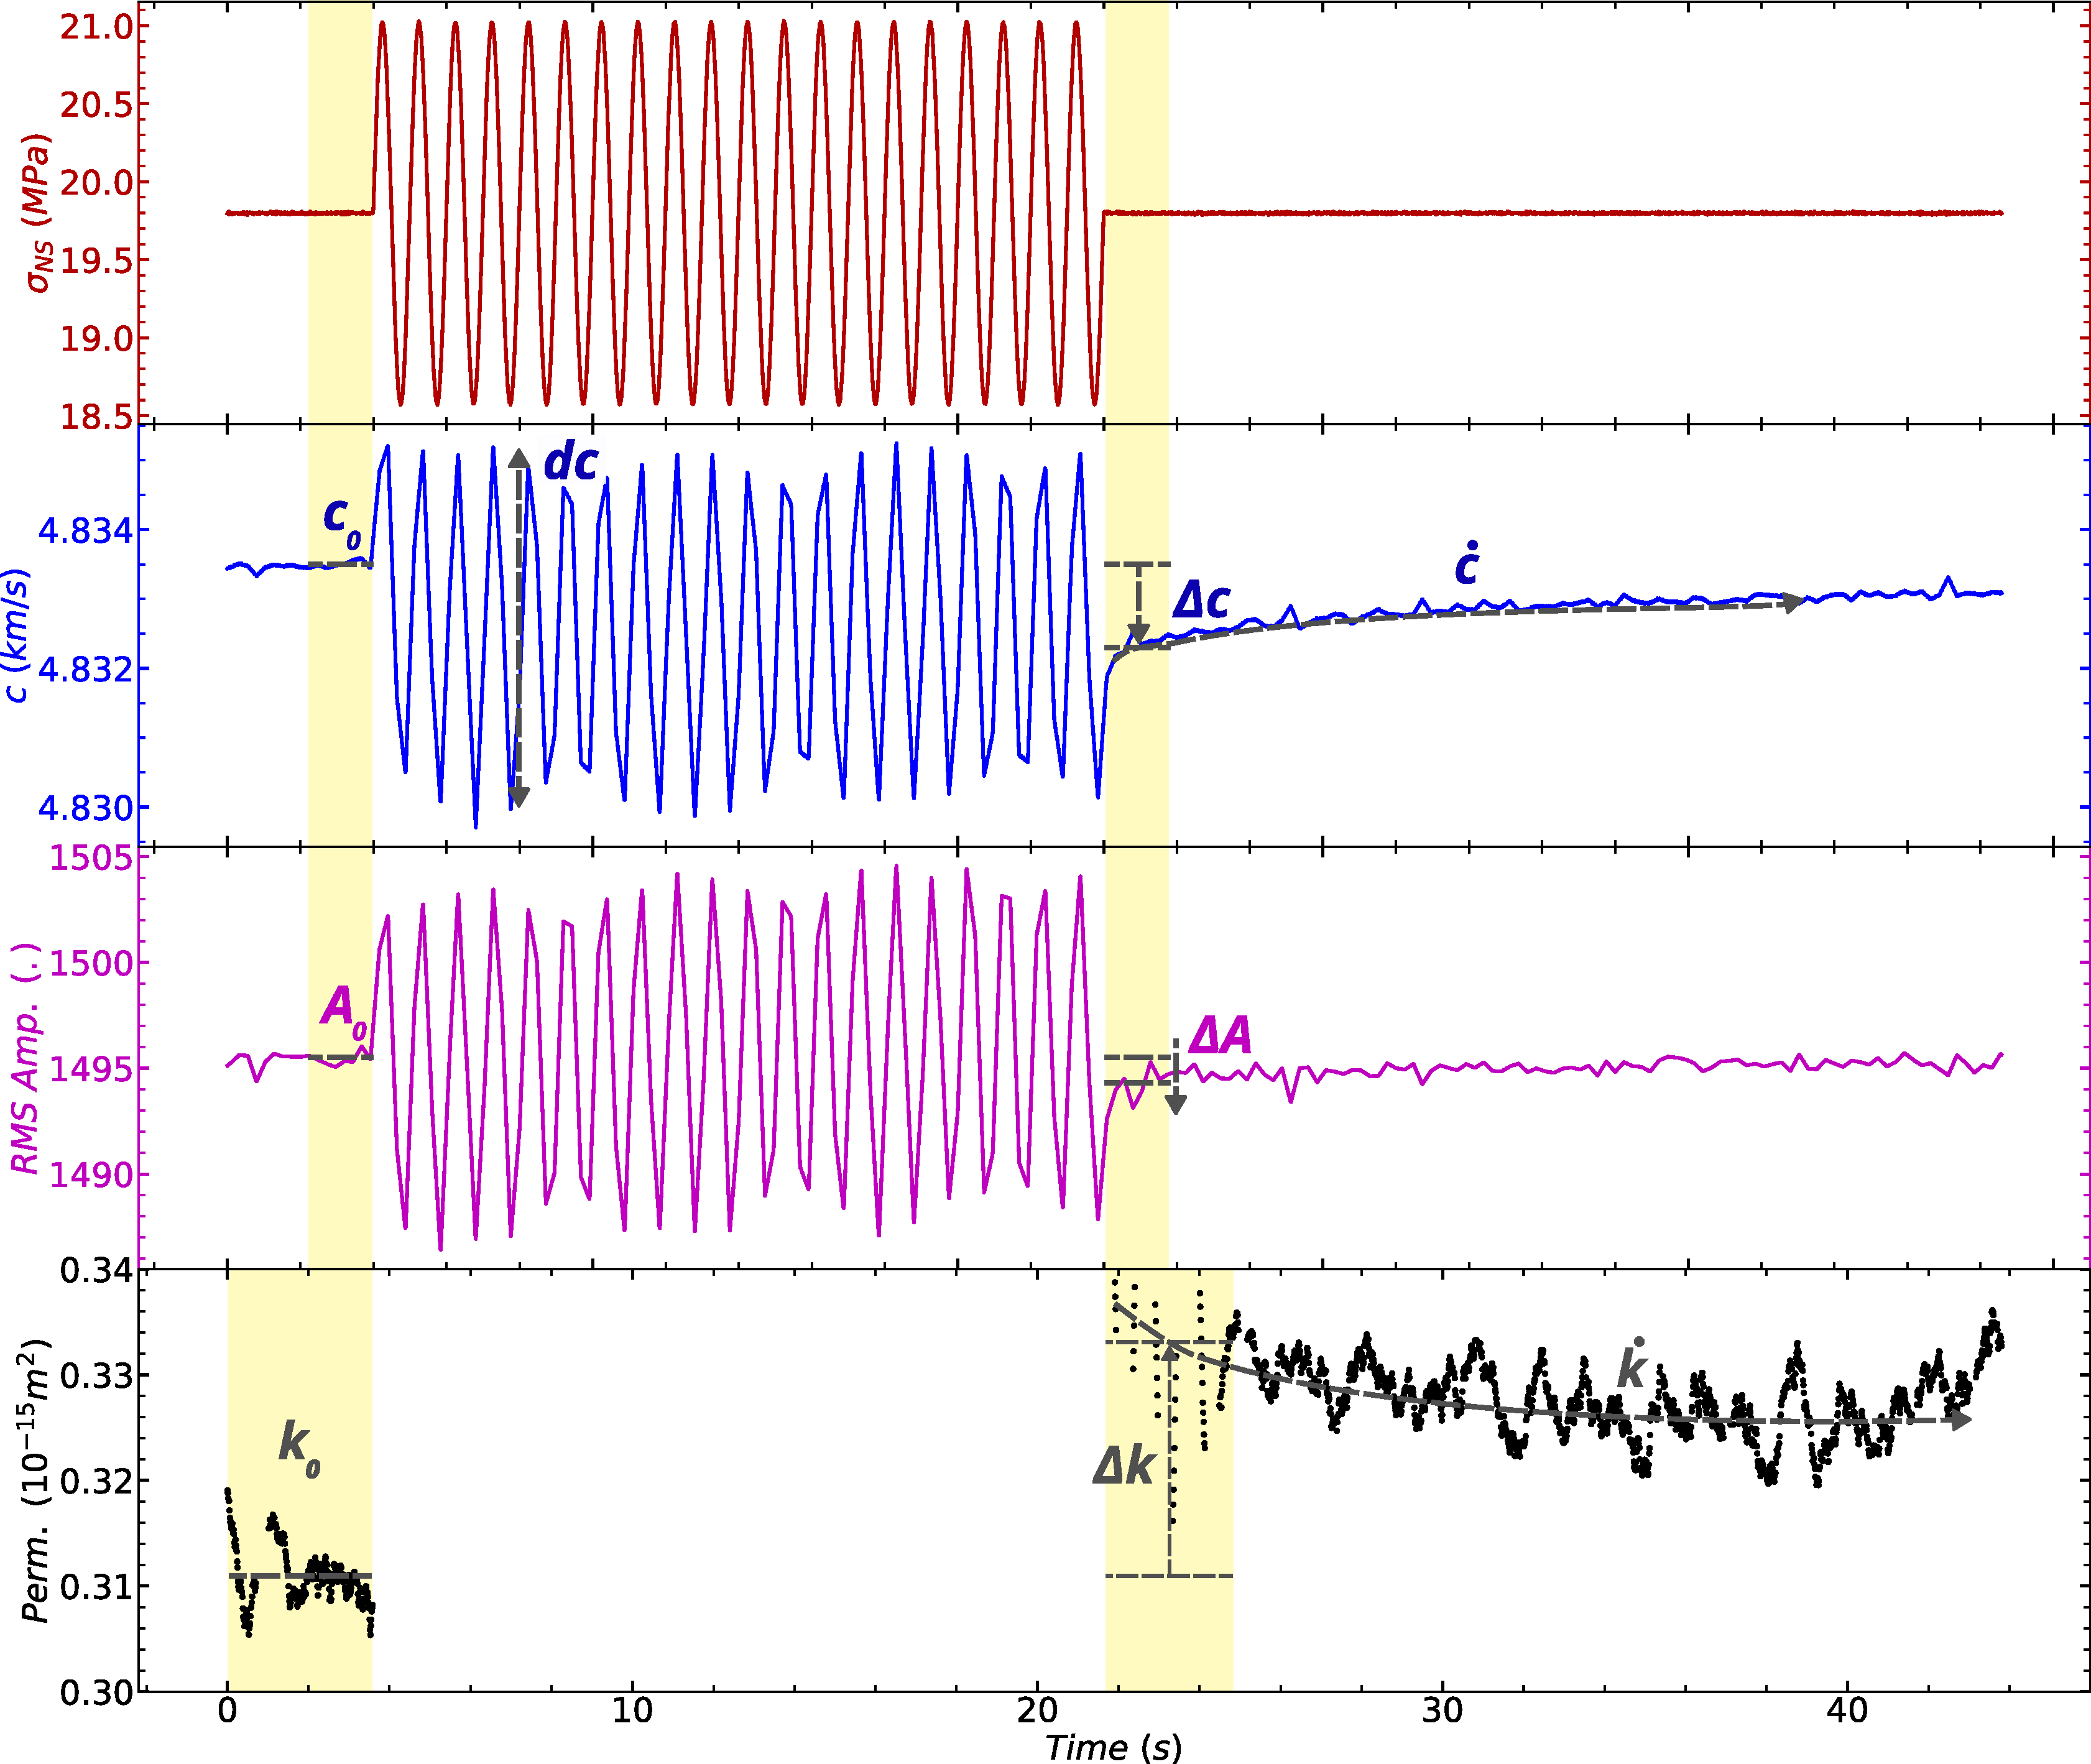
\includegraphics[width=0.9\columnwidth]{NsVelRmsPerm_edit}
	\caption[]{The velocity and permeability changes are calculated using the measured values before and after each oscillation averaged over the time windows (gray boxes) shown in (c). Data points in the permeability measurements are omitted on the condition that inlet/outlet flow rates differ $ > 5 \% $. That is to say, plotted permeability points represent when there is steady-state flow, necessary for Darcy’s law. Dashed lines indicate the recovery of p-wave velocity ($ \dot c$) and permeability ($\dot k$), respectively, from post-oscillation response to new steady-state value. Furthermore, we parameterize the p-wave velocity change $ dc $ during the normal stress or pore pressure oscillations, indicated by dashed blue line.}
	\label{fig:delc_delk_calc}
\end{figure*}

\newpage

\begin{figure}[ht]
	\centering
	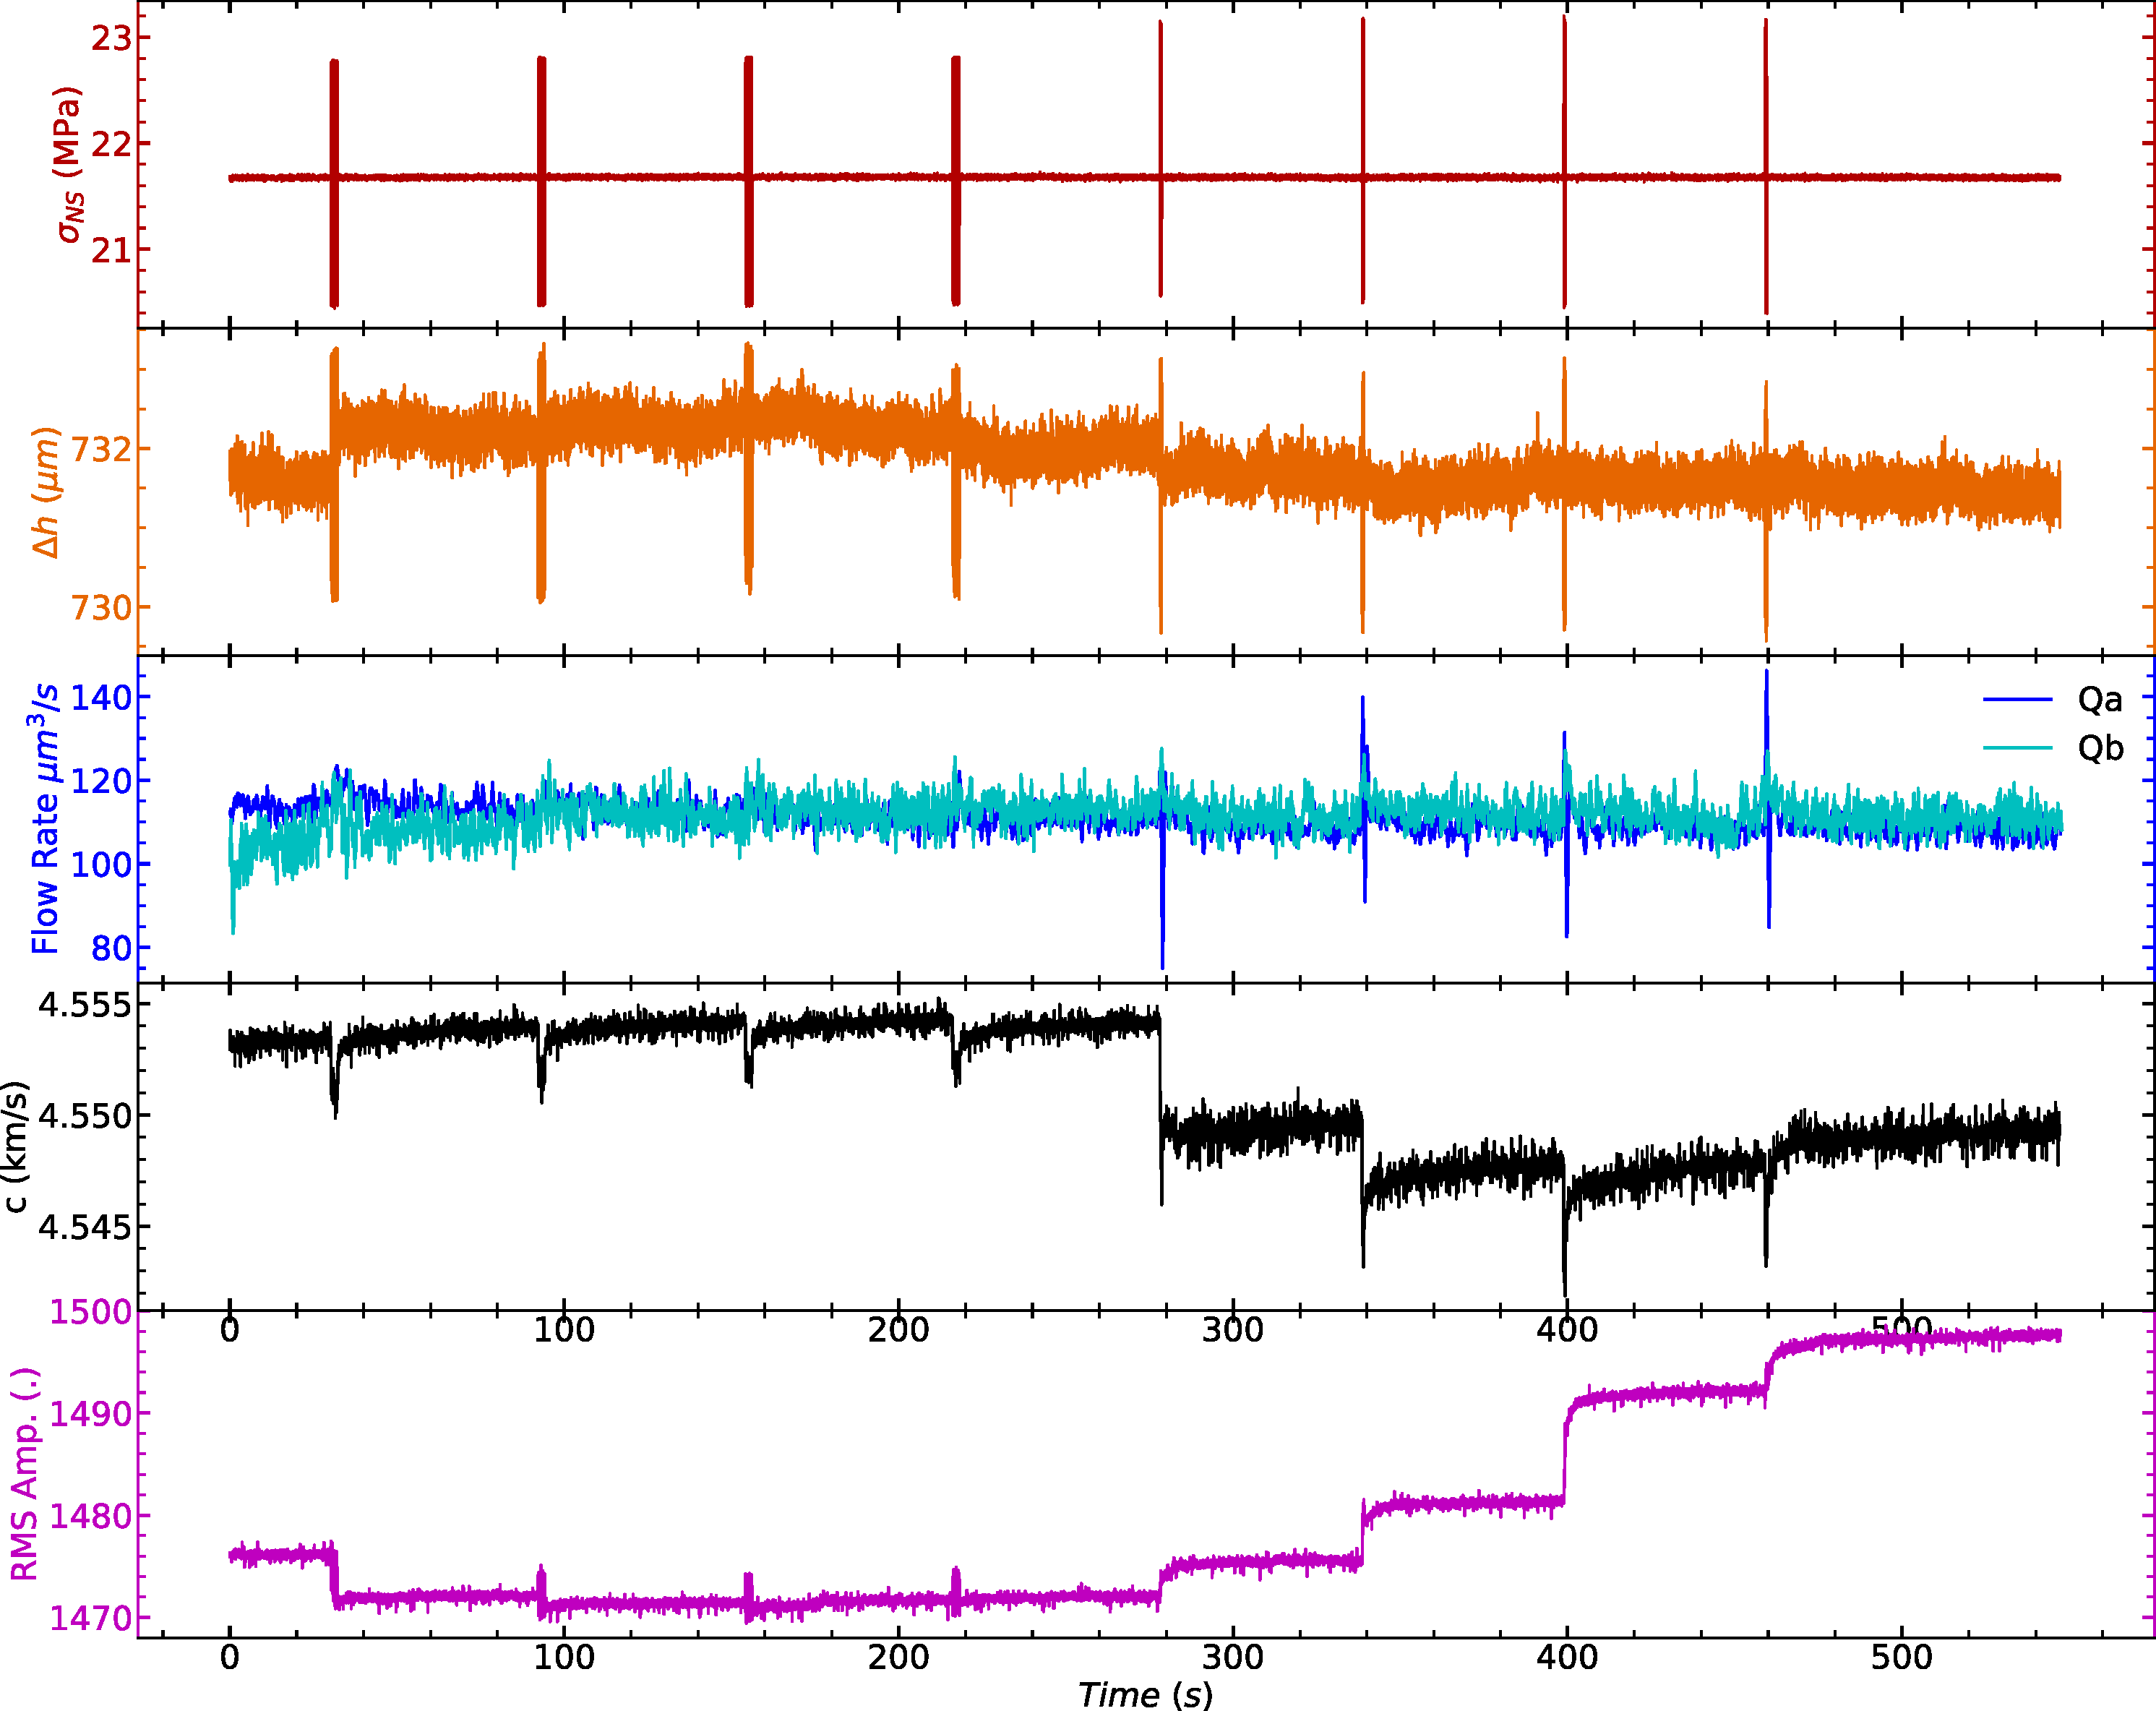
\includegraphics[width=1\columnwidth]{NS_p4975_run4}
	\caption{Run 4 of experiment p4975.}
	\label{fig:run4_p4975}
\end{figure}

\newpage


%\paragraph{}
%The details on amplitude- and frequency-dependencies of 
%delc/c0 and dc/c0 for a single transmitter-receiver pair are given in Shokouhi et al. (2019). Similar trends are observed for all transmitter-receiver pairs and therefore, not repeated here. In summary, the results given in Shokouhi et al. (2019) indicate that delc/c0 and 
%dc/c0 are modulated by dynamic stress amplitudes for both pore pressure oscillations and fracture normal stress oscillations (Figure 3 and Figure 4). In addition, the measurements exhibit frequency-dependence (not shown here); delc/c0 increases with the oscillation frequency, while dc/c0 mostly decreases. Observing different trends for the different nonlinearity parameters is not surprising. Although the origins of delc/c0 and dc/c0
%remain unclear, there is empirical evidence that they stem from different micro-mechanical mechanisms (Riviere et al., 2016, 2015). 
%Although the c. values tend to generally increase with the oscillation amplitude, we do not observe a clear trend (not shown). This could be in part due to the variability in 
%c. caused by the low signal-to-noise ratio. The recovery rate c. does not show a systematic dependency on frequency (not shown).  
%\paragraph{}
%Shearing of the fracture reduces dc/c0 during normal stress oscillations (Figure 4a). Interestingly, we have recorded different post-shear behavior for normal stress vs. pore pressure oscillations; the shearing increases the nonlinearity during pore pressure oscillations for one sample (p4975), while decreasing it for the other sample (p4966) (Figure 4b). This and other observations indicate possible differences in mechanisms activated during these two modes of dynamic stressing. On the other hand, shearing does not have a significant influence on delc/c0. The second shearing step decreases the measured nonlinearity delc/c0 but only slightly.
%
%\newpage

\begin{figure*}[h]
	\centering
	%	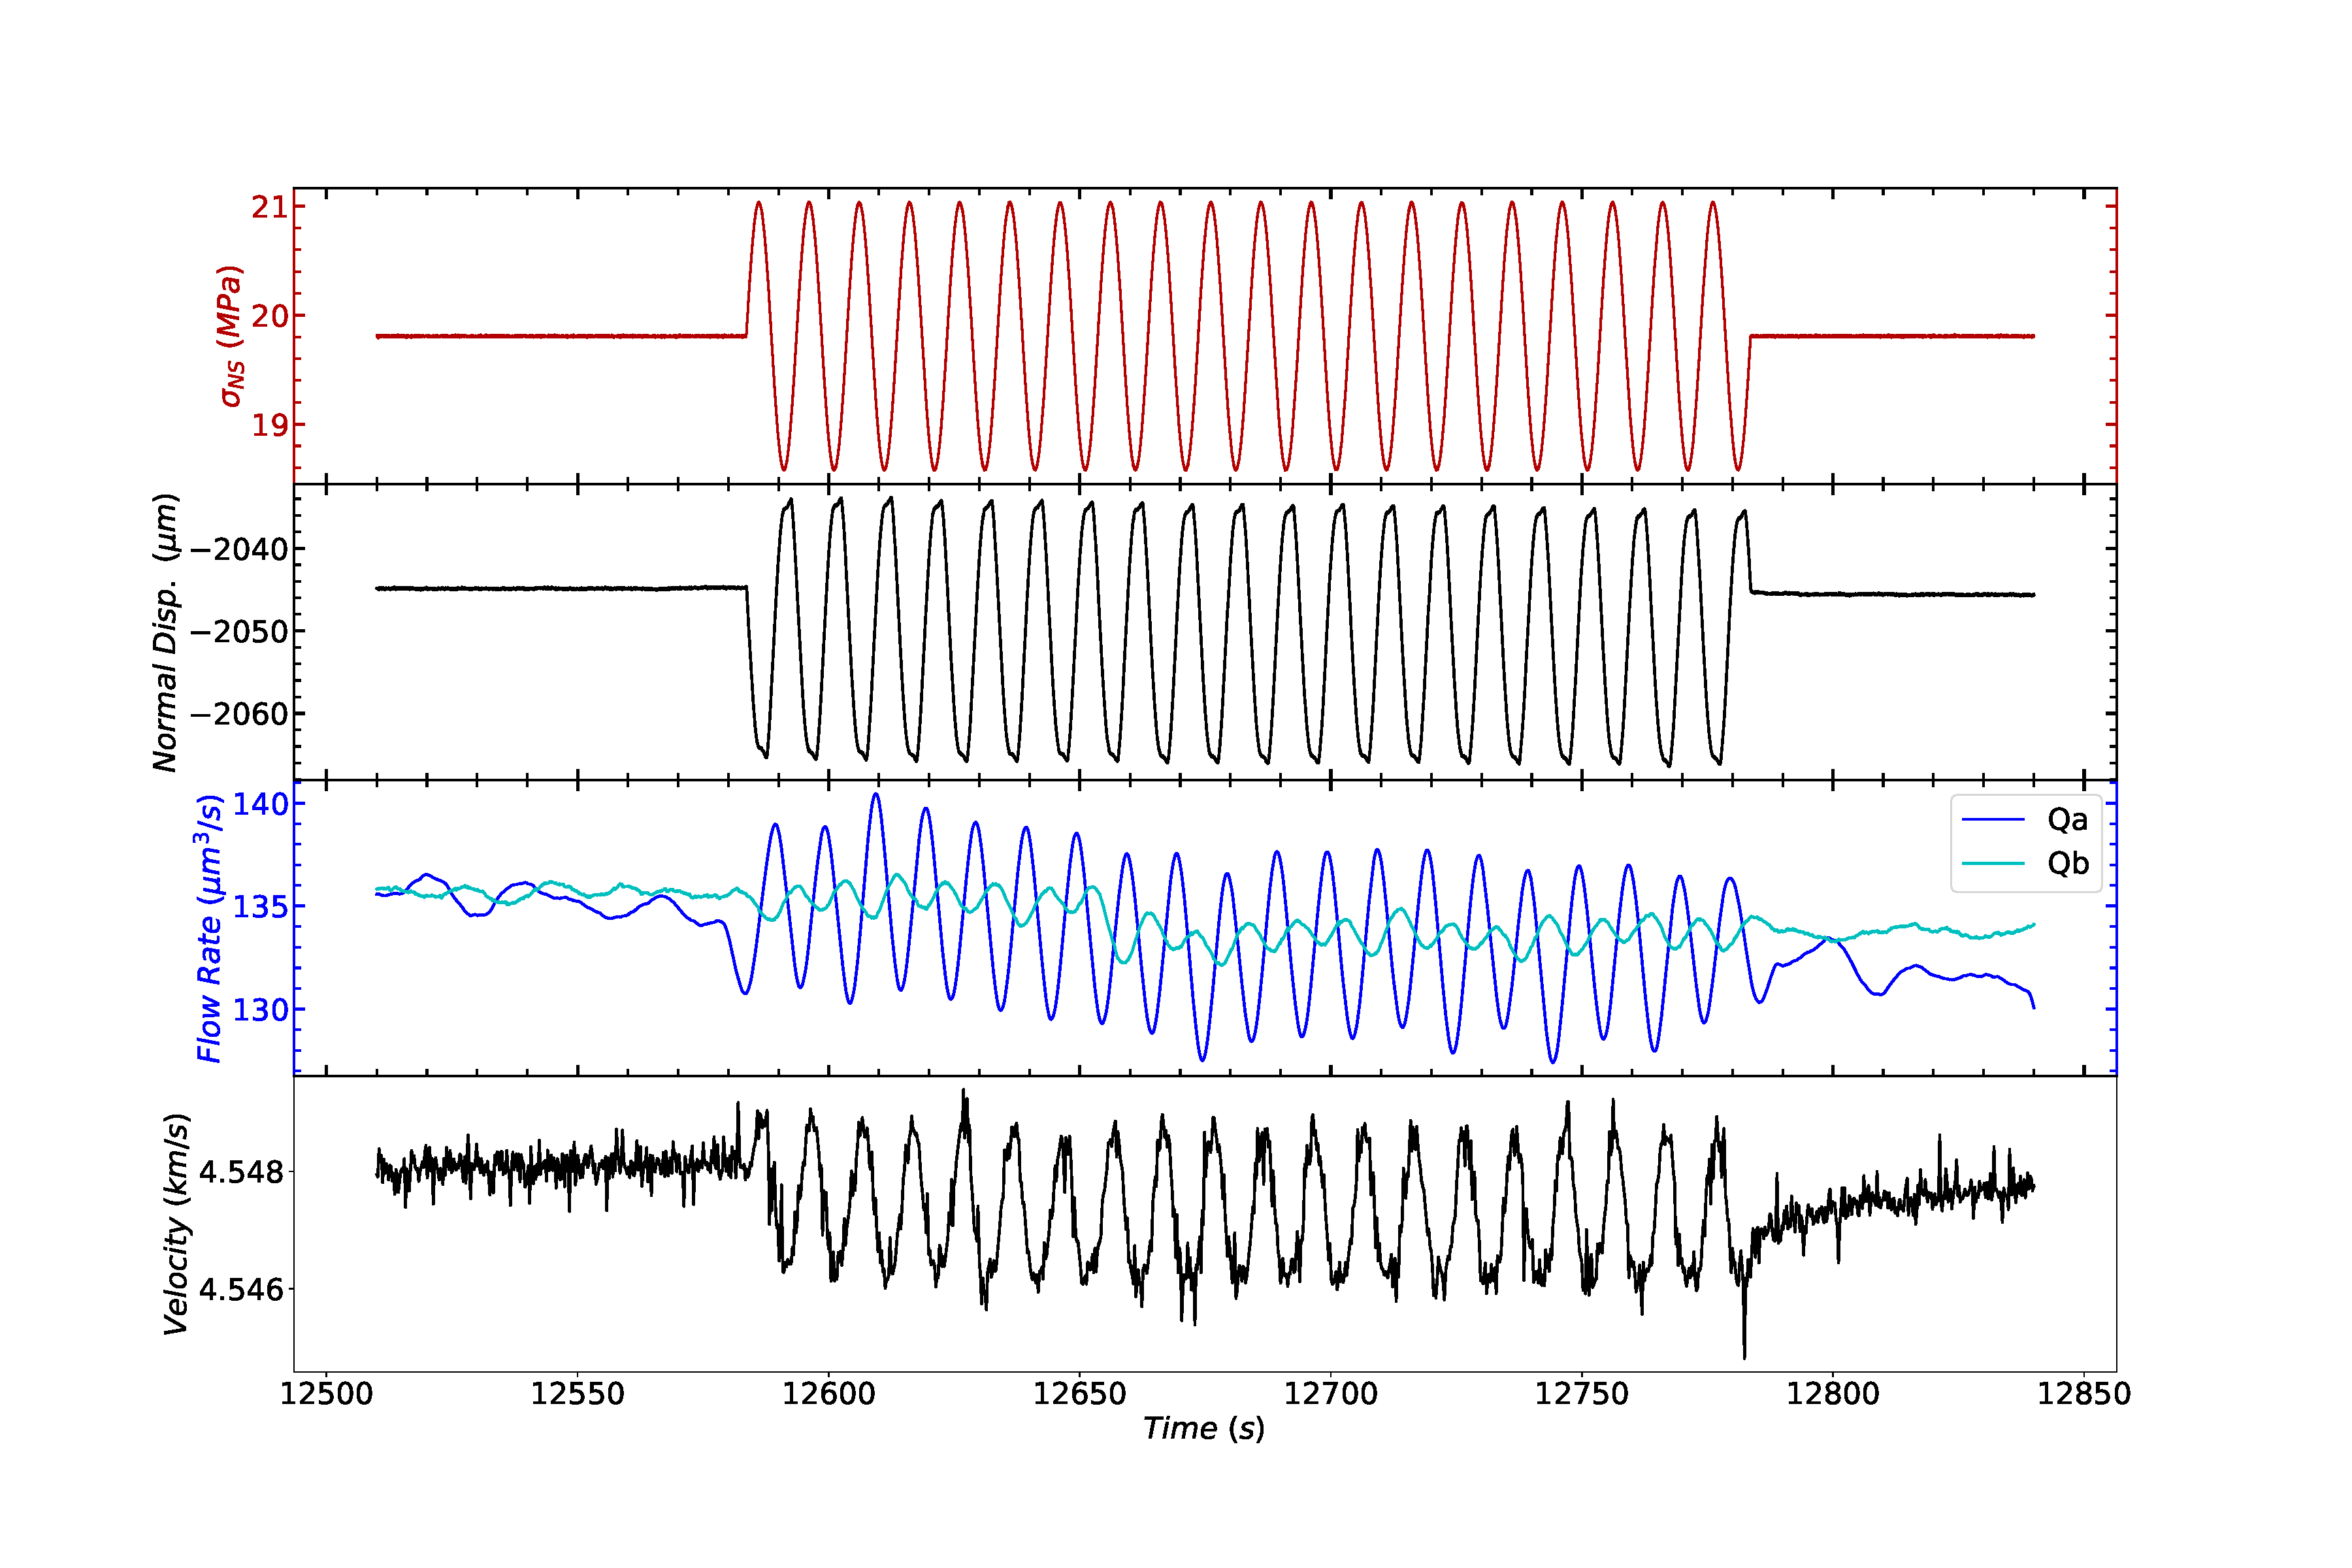
\includegraphics[width=0.8\columnwidth]{NS_p4975_run3b_01Hz}
	%	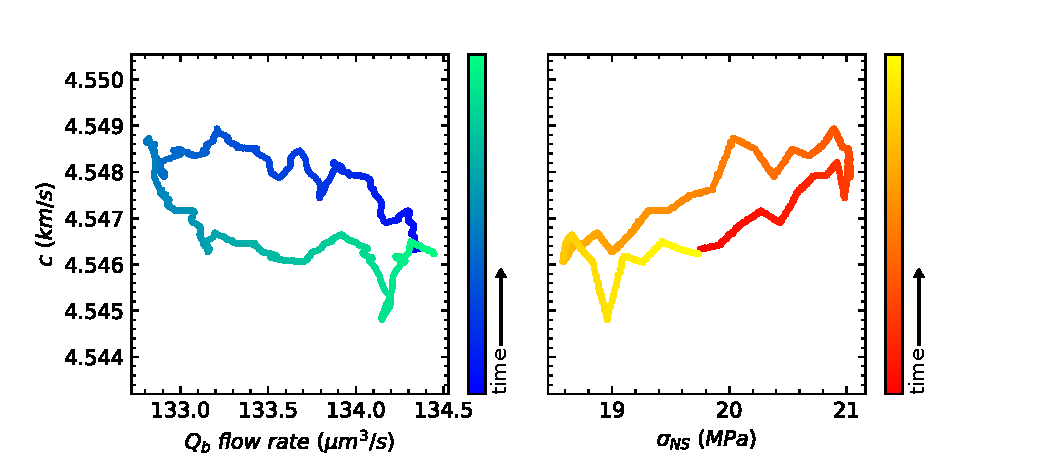
\includegraphics[width=0.7\columnwidth]{NSbowtie_p4975_run3b_01Hz_Cycle19}
%	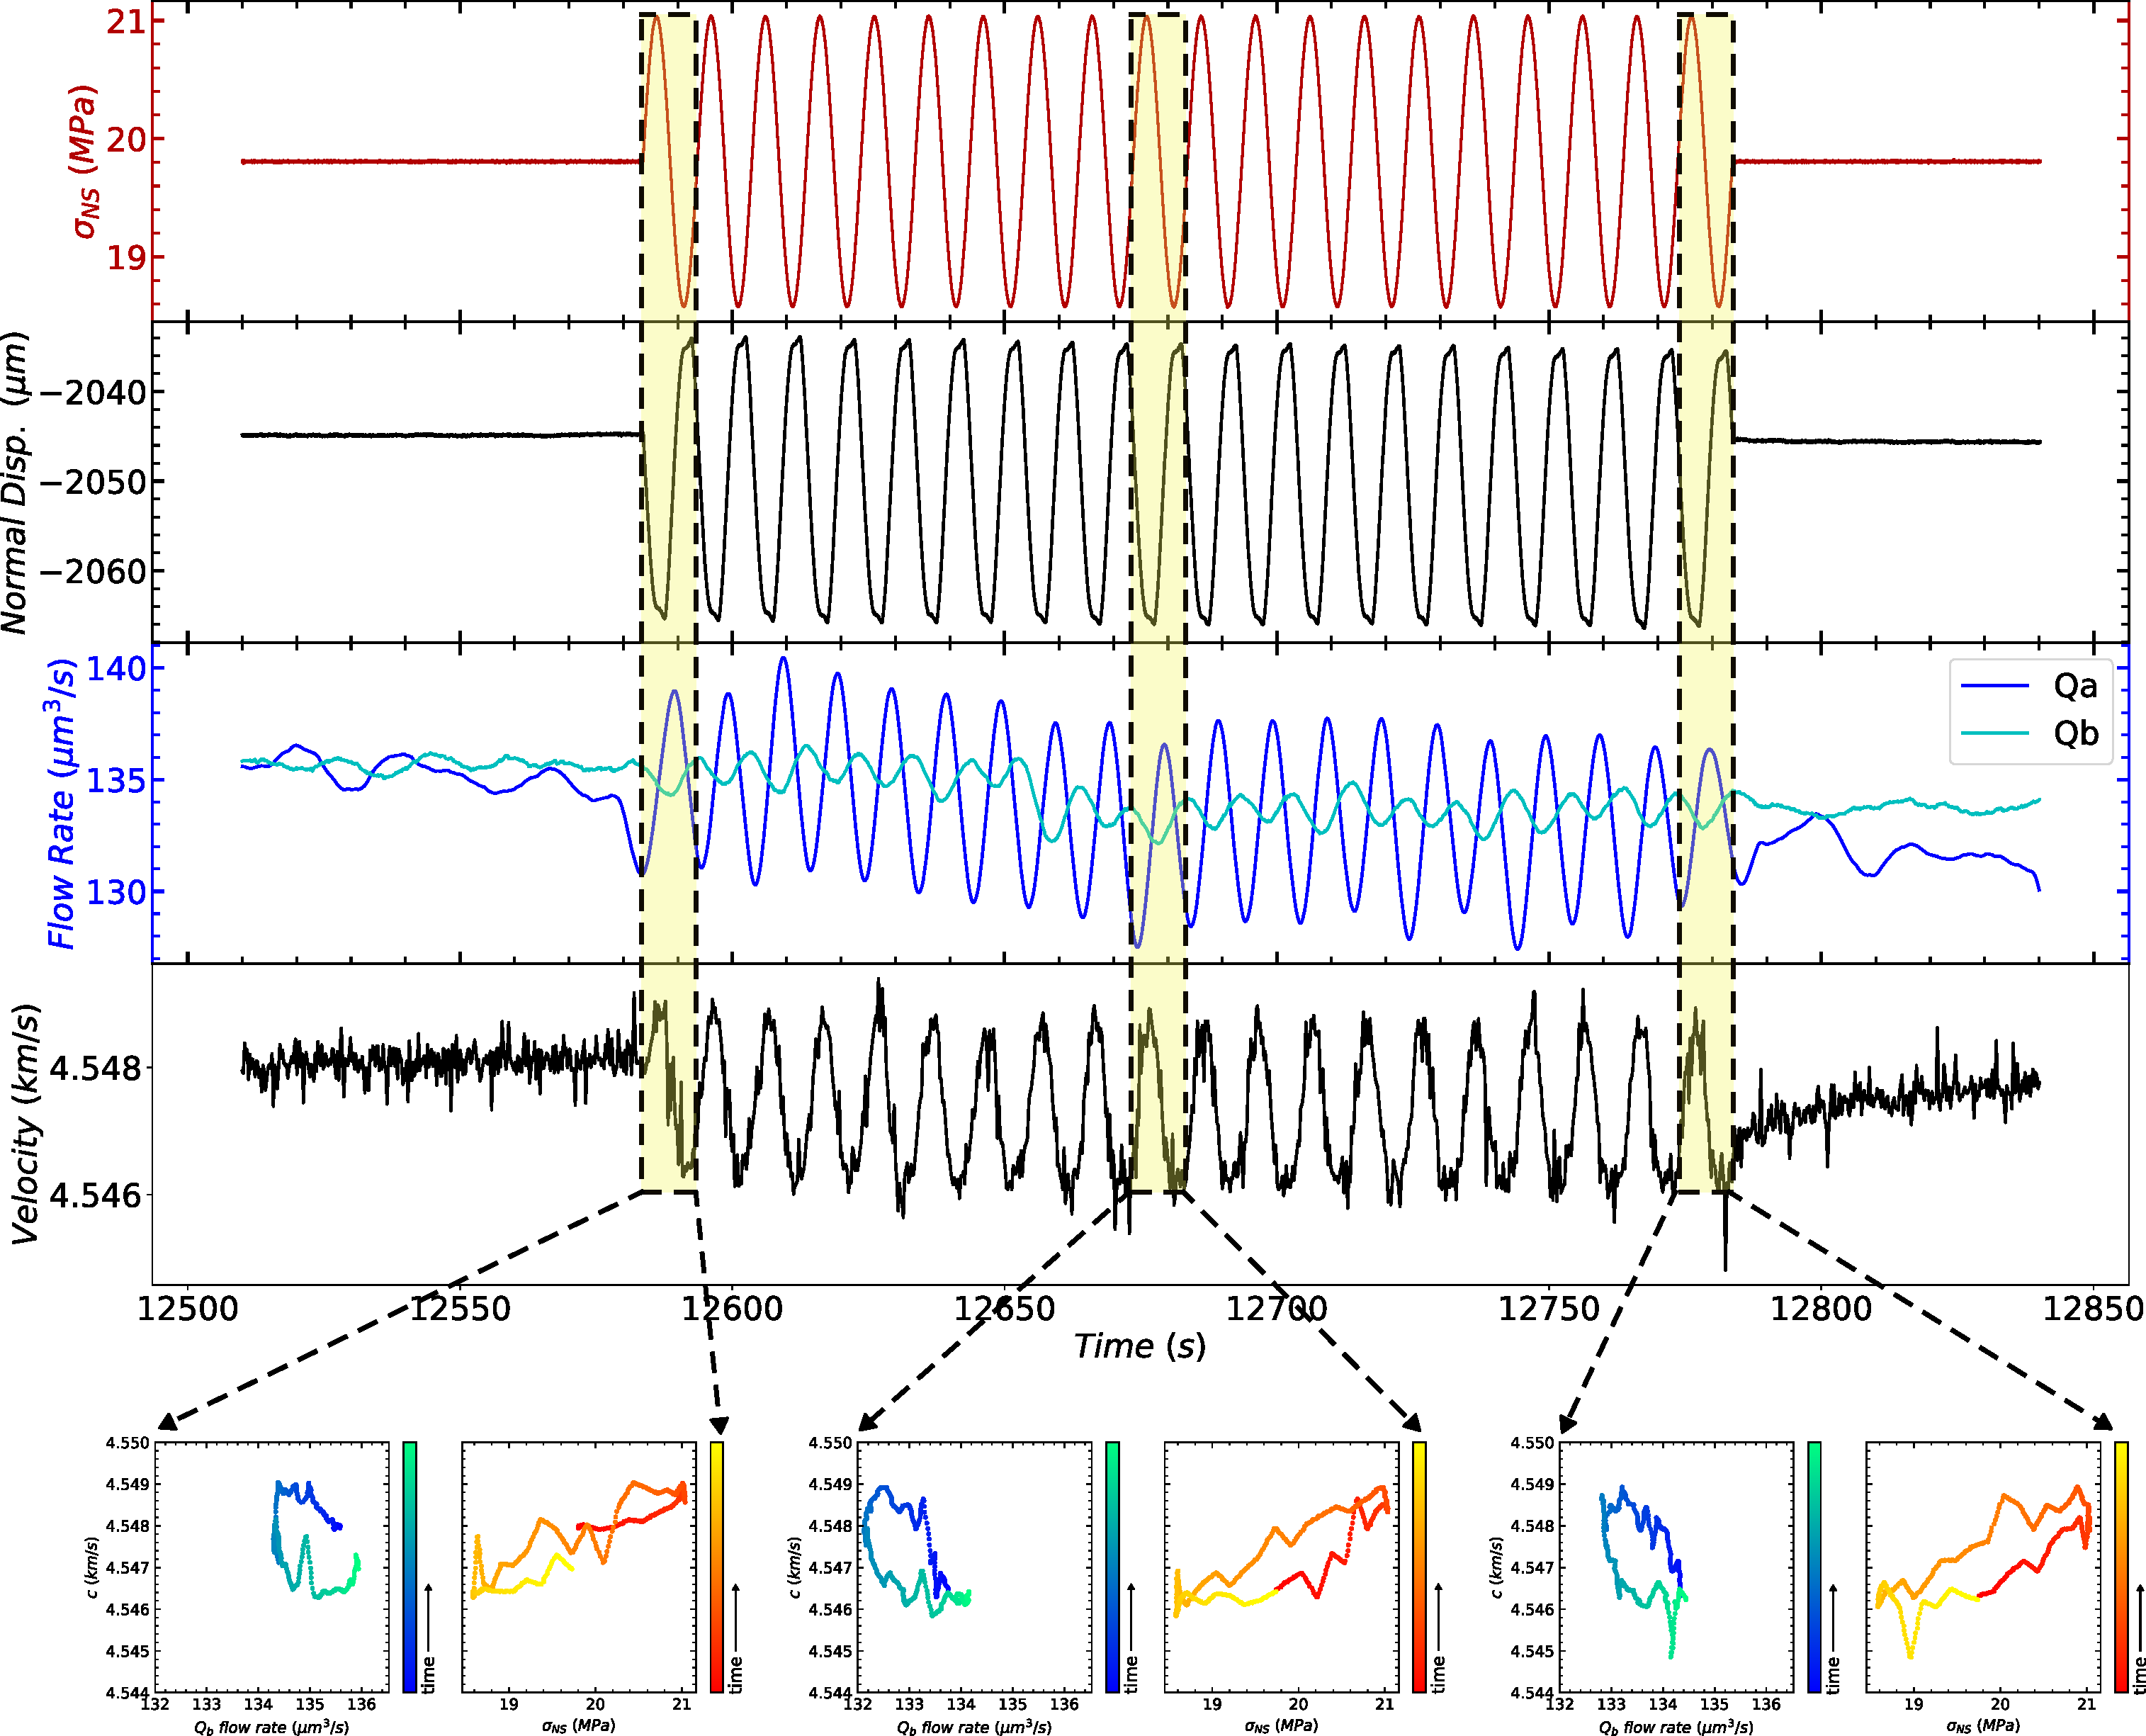
\includegraphics[width=0.99\columnwidth]{NS_bowtie_p4975_run3b_01Hz}
	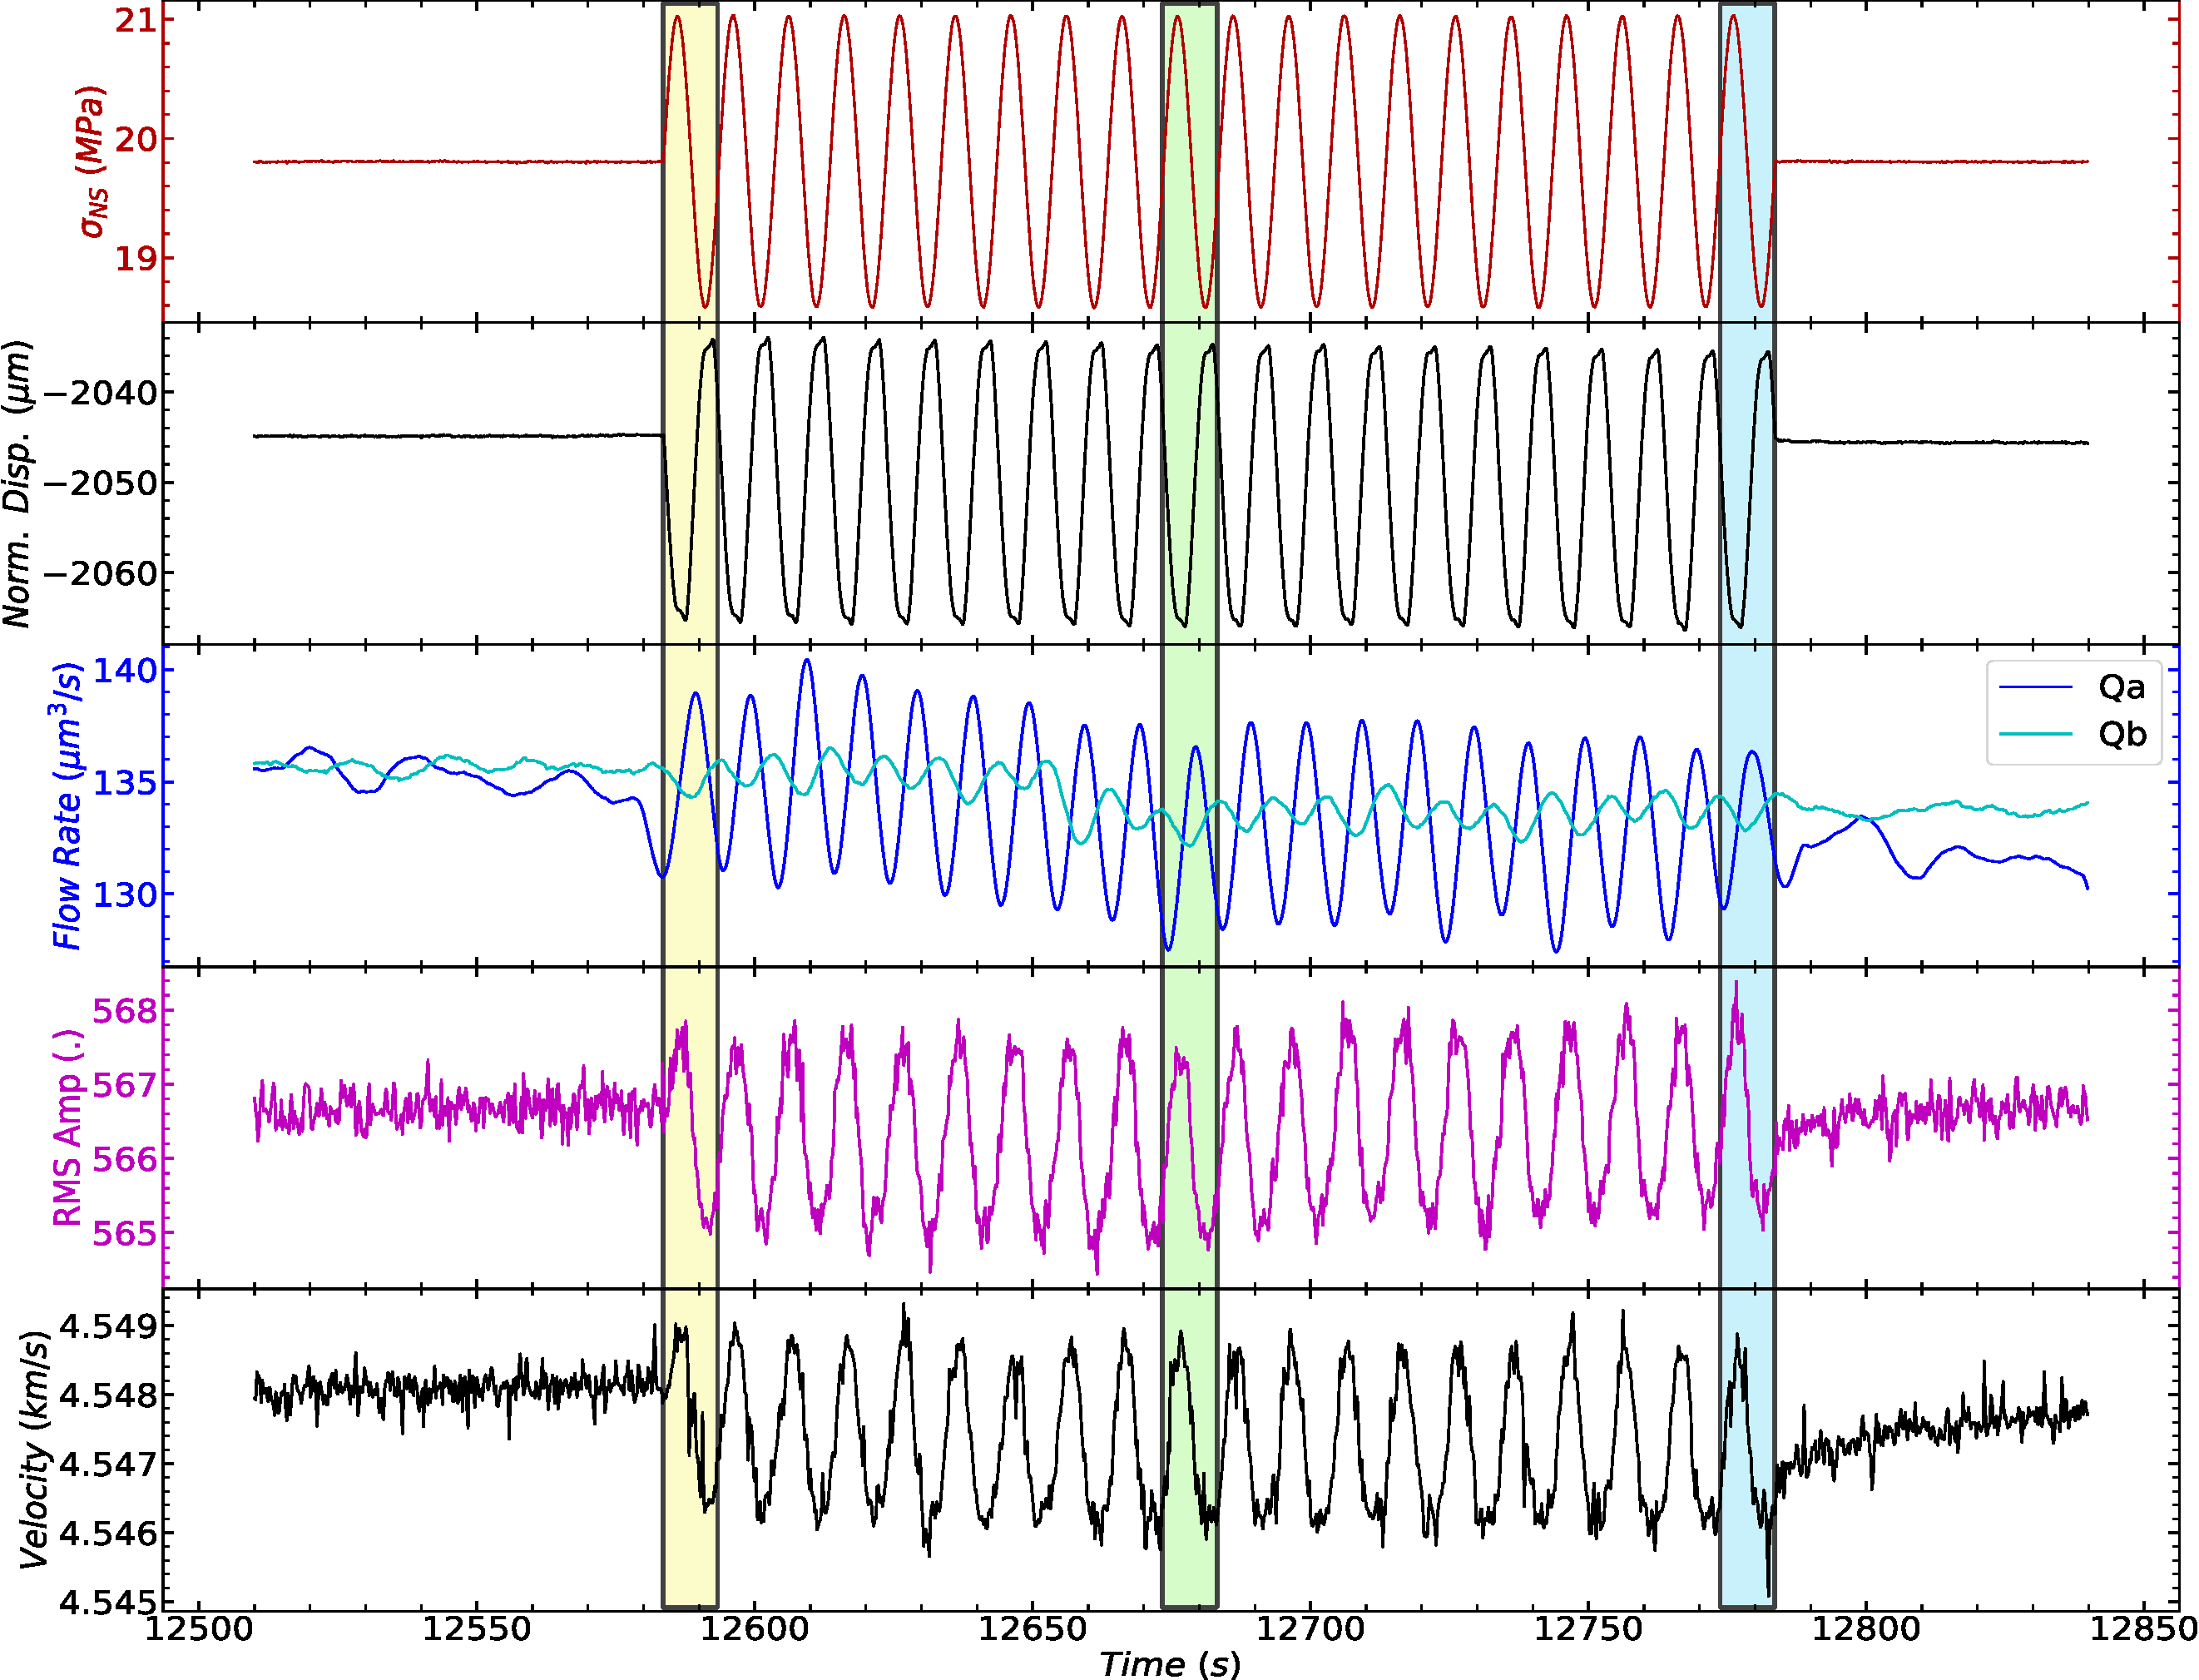
\includegraphics[width=0.8\columnwidth]{plots_bowtie_p4975_run3b_01Hz}
	\caption[]{Direct response of normal displacement, flow rate (inlet and outlet), and ultrasonic RMS amplitude and velocity for the direct path pair during a 0.1Hz 1MPa Normal Stress oscillation. Note the phase delay between the inlet and outlet flow rates. Three sections are highlighted showing one full cycle in the beginning, middle, and end of the normal stress oscillation. }
	\label{fig:NS_p4975_run3b_01Hz}
\end{figure*}

%\textcolor{red}{Delineate (b) \& (c) to distinguish compression and tension of oscillation.\\}

\newpage

\begin{figure*}[ht]
	\centering
	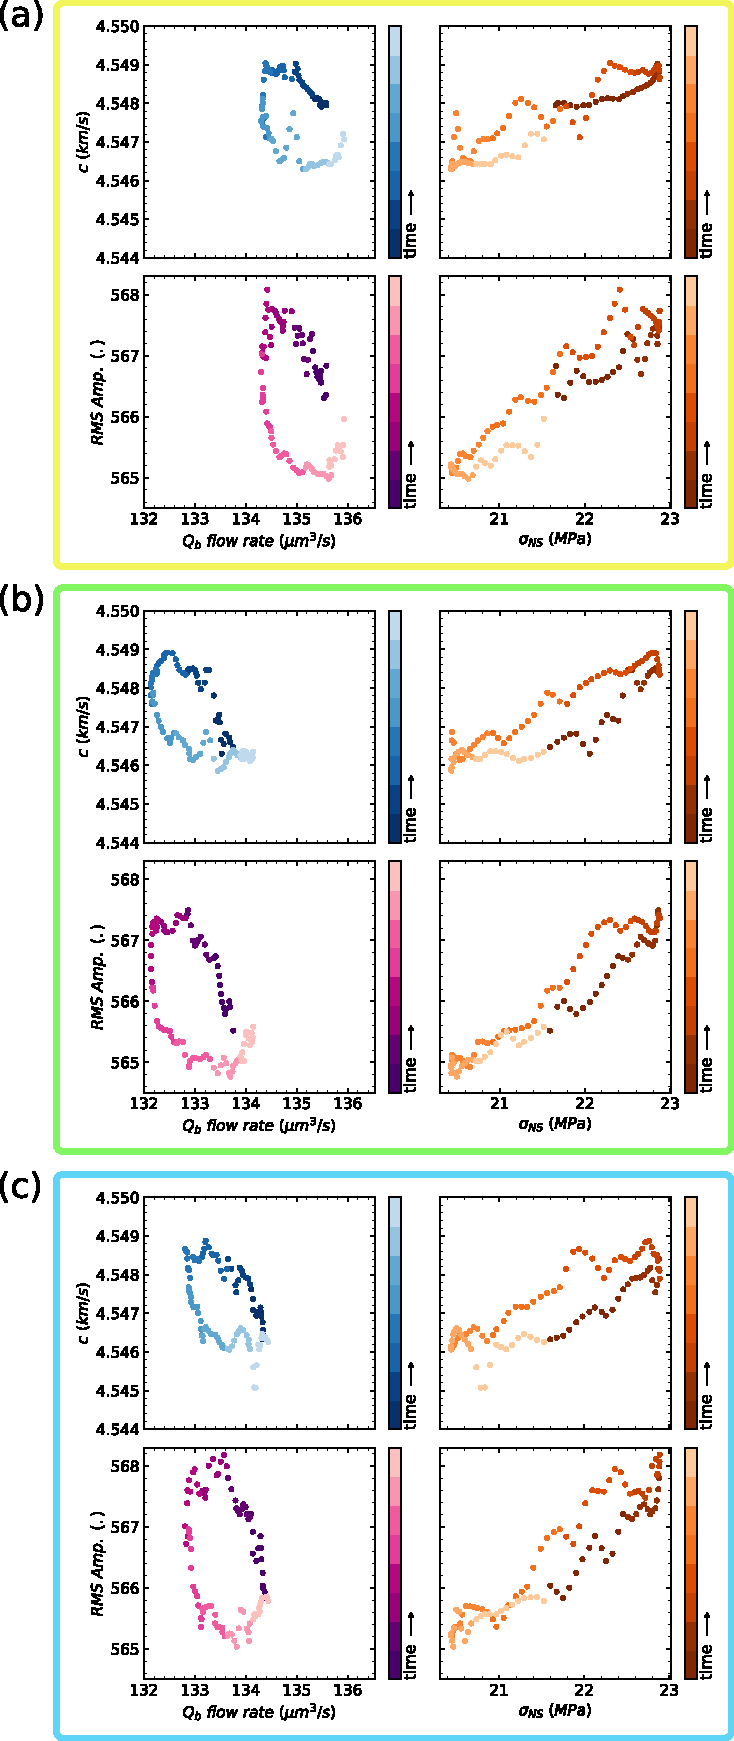
\includegraphics[width=6.0cm]{bowtie_p4975_run3b_01Hz_v2}
	\caption[]{Evolution of the fracture during a 1 MPa, 1 Hz normal stress oscillation during the first cycle (a), middle cycle (b), and last full cycle (c). The relationship between velocity and RMS Amplitude with outlet flow rate track each other throughout the oscillation, ending in decreased flow. The point to make here is that the fracture is continuously changing -- the change in aperture results in change in velocity and flow paths.}
	\label{fig:bowties}
\end{figure*}


\newpage

%\subsection{perm evolution}
%\paragraph{perm evolution: transient response to dynamic stressing \& shear:} 


%\paragraph{Oscillation Amplitude- and Frequency-Dependencies:} 
%The dependencies of delk/k0 on the amplitude (Figure 5) and frequency of normal stress and pore pressure oscillations are given in Shokouhi et al. (2019). One important observation is that although small-amplitude oscillations ($< $ 0.5MPa) may result in a decrease in permeability, large-amplitude oscillations generally increase permeability transiently. Furthermore, for the same oscillation amplitude and frequency, the pore pressure oscillations appear to be more effective in permeability enhancement (delk/k0 $> $ 0) than the normal stress oscillations by a factor of ~2.5, particularly for sample WG1. In addition, delk/k0
%increases, albeit slightly, with the frequency of oscillations (not shown here). The only exception is the decrease in delk/k0 for sample WG2, when we increase the fluid pressure oscillations from 1 Hz to 10 Hz. The details on amplitude- and frequency-dependencies of 
%delk/k0 are given in Shokouhi et al. (2019). The recovery rate k. does not show clear amplitude- and frequency-dependencies (not shown here).  
%
%\paragraph{Influence of Shearing:}
%Generally speaking, after shearing the fracture, the normal stress oscillations become less effective in enhancing the fracture permeability (see Figure 5a). The trend is less obvious for pore water pressure oscillations (see Figure 5b). 
%
%\paragraph{correspondence b/w stiffness \& perm transients:}
%The main hypothesis driving this study was that the transient elastic softening is associated with a temporary increase in porosity and/or permeability, both of which are important for energy production and waste storage. Our results to date support this conjecture: the relative changes in wave velocity and permeability of fresh fractures (before shearing), due to both normal stress and pore pressure oscillations, are correlated, such that a larger drop in wave velocity (more negative delc/c0, equivalent to larger transient softening or higher nonlinearity) corresponds to a larger permeability enhancement delk/k0.  As shown in Figures 6a and 6b (left panels), this overall correlaltion seems to hold for both normal stress and pore pressure oscillations. Furthermore, the recovery rates of wave velocity and permeability transients (c. and k.) also seem to be correlated (Figure 7), although there is slightly more scatter. This observation further reinforces the presumed linkage between the evolution of fracture's elastodynamic and flow properties. In other words, the form of the measured permeability transients is similar to that for the nonlinear elastic effects and both recoveries follow the time-logarithmic trajectories observed in the field or in nature. We should note that the correlations shown in Figure 6 correspond to delc/c0 averaged for 5 transducer pairs shown in Figure 1d. Examining the results for individual transducer pairs (not shown here) reveals the strong dependency of the measurements on the wave path. This is not surprising as the fracture aperture is nonuniform and the ray paths sample different portions of that interface. 
%
%Shearing the fracture appears to alter these relations indicating the influence of contact stiffness and shear fabric on both sets of properties (Figure 6a and 6b). Overall, shearing seems to weaken the correlation between delc/c0 and delk/k0 (Figure 6a and 6b, middle and right panels). The question remains as to what underlying micro-mechanisms link the nonlinear elastodynamic behavior and hydraulic properties of fractures. 
%
%We considered two mechanisms for this observed correspondence: (1) the unclogging of fracture flow conduits via fluid pressure oscillations, and (2) the dependence of both properties on stress-induced changes in the fracture aperture. Previous work shows that particle clogging can alter permeability via dynamic stressing in Berea sandstone (Elkhoury et al., 2011; Candela et al., 2014, 2015). However, for fractures in Westerly Granite we observe an increase in permeability for both pore pressure and normal stress oscillations of sufficiently large amplitude. With the new insights from the coupled ultrasonic data, one may conclude that unclogging is merely one of many potential mechanisms. 
%
%The other explanation for the linkage between stiffness and flow properties of fractured rocks could be the dependence of both properties on the fracture aperture change due to the imposed stress oscillations. To further examine this hypothesis, we investigated whether 
%delc/c0 or delk/k0 correlate with the measured changes in sample thickness changes (proxy for aperture compaction/dilation) during imposed oscillations (Shokouhi et al., 2019). However, we did not observe a strong correlation. This lack of strong correlation suggests that changes in fracture aperture cannot be the sole driving mechanism for permeability change, especially when driven by pore pressure oscillations.  
%
%We also used high-resolution optical profilometry to measure the roughness across the post-mortem fractured surfaces in order to reconstruct the fracture aperture distribution. However, since the fractures were created in-situ and were sheared twice before the roughness measurements, we do not have information on the aperture or roughness of fracture interfaces immediately post-fracture nor immediately post-shear (1st shearing step).  
%
%\newpage

%\paragraph{From Prabaha's Arma:}
%The nonlinear parameter delc/c0 is plotted against the applied normal stress oscillation amplitude (0.2-1MPa) in Figure 5. The sample is more nonlinear if the absolute value of 
%delc/c0 is larger at a given oscillation amplitude and frequency. As shown in Figure 5 (a) 
%delc/c0 of the intact sample increases as the normal stress amplitude increases. Also, the nonlinearity seems to increase with the oscillation frequency. This trend closely resembles previous observations in dry intact Berea sandstone (Riviere et al., 2016). Similar trends are observed for the fractured sample in dry (Figure 5 (b)) and saturated (Figure 5 (c)) states. The results for the saturated fractured sample at 1Hz are also comparable to our previous observations on in-situ-stressed fractured samples of Westerly granite (Shokouhi et al., 2019).  
%
%We observe that the saturated fractured sample exhibits less nonlinearity than both the dry intact and fractured samples. For an intact sample, saturation decreases the pore compressibility, which increases wave velocity (Winkler and McGowan, 2004) and decreases nonlinearity (Ostrovsky and Johnson, 2001; Van Den Abeele, 2002). A decrease in the nonlinearity of an intact saturated rock sample has also been reported by Van den Abeele et al, 2002, Johnson et al., 2004 using a resonance-based method. For  the saturated fractured sample, the decrease in the measured nonlinearity is due to the presence of the fluid and the resulting increased interface stiffness (Dwyer-Joyce, Zhu and Reddyhoff, 2010; Ooi and Dwyer-Joyce, 2016). 
%\paragraph{}
%Figure 7 shows the normal stress amplitude- and frequency-dependency of the second extracted nonlinearity parameter dc/c0 for the sample in the three states. Similar to delc/c0, dc/c0
%scales linearly with amplitude although, the trend here is clearer. A linear dependency is also apparent in dry intact Berea sandstone (Riviere et al., 2015). In addition, there is no discernible dependency on the frequency of oscillations. This observation aligns with that reported in a previous study (Riviere et al., 2016), where dc/c0 or the second harmonic amplitude was observed to be independent of the imposed oscillation frequency. Similar to what was observed for delc/c0, the dry intact sample appears more nonlinear than the dry fractured sample, which exhibits more nonlinearity than the saturated fractured sample.  

%\newpage


\subsection{Nonlinear Elastodynamic Response: Relative Change in Permeability and Velocity}
\paragraph{}
%The main hypothesis driving this study was that the transient elastic softening is associated with a temporary increase in porosity and/or permeability, both of which are important for energy production and waste storage. Our results to date support this conjecture: the relative changes in wave velocity and permeability of fresh fractures (before shearing), due to both normal stress and pore pressure oscillations, are correlated, such that a larger drop in wave velocity (more negative delc/c0, equivalent to larger transient softening or higher nonlinearity) corresponds to a larger permeability enhancement $ \Delta k/k_0 $.  As shown in Figures 6a and 6b (left panels), this overall correlation seems to hold for both normal stress and pore pressure oscillations.

The relative change in permeability $ \Delta k/k_0 $ is defined as the change in permeability resulting from imposed normal stress or pore pressure oscillations, normalized to the pre-oscillation permeability (Candela et al., 2014). Figure \ref{fig:delc_delk_calc} shows the pre-oscillation permeability $ k_0 $ and the post-oscillation permeability $ k = k_0 + \Delta k $ are calculated by averaging the measured values over 10- and 1-s time windows. Calculation discontinuities in permeability measurements shown in Figure SXX correspond to the data points for which inlet/outlet flow rate difference exceeds the 5\% threshold. 

\paragraph{}
The dependency of $ \Delta k/k_0 $ on the amplitude and frequency of normal stress and pore pressure oscillations are shown in Figure \ref{fig:perm_ns_amp}. The red dashed lines in these figures at $ k = k_0 + \Delta k $ mark the boundary between permeability increase and decrease due to the imposed oscillation. Despite the scatter in the data (Figures 4a and 4b),the relative permeability change $ \Delta k/k_0 $ generally scales with the amplitude of 1‐Hz normal stress and pore pressure oscillations. Small‐amplitude oscillations may even result in a decrease in permeability, where as large‐amplitude oscillations generally increase the permeability. Comparatively, pore pressure oscillations appear to be more effective in enhancing permeability $ \Delta k/k_0 > 0$) than normal stress oscillations. The frequency dependence of permeability changes for normal stress and pore pressure oscillations. Note that the permeability changes are larger for the 10‐Hz fluid pressure oscillations as well as the 40‐Hz normal stress oscillations.The permeability change increases slightly with frequency. The only exception is the decrease in $ \Delta k/k_0 $ for WG2, when we increase the fluid pressure oscillations from 1 to 10 Hz.
%\begin{itemize}
%	\item nonlinearity modulated by oscillation amplitudes
%\item nonlinearity and permeability enhancement generally increase with frequency of dynamic stressing.
%\item relative changes in wave velocity and permeabilityare correlated: larger drops in velocity —> larger increases in permeability
%\item changes in permeability are greater at higher oscillation amplitudes 
%\subitem Perm enhancement pronounced for Pp oscillations than for NS.
%\end{itemize}

%\paragraph{}
%The dependencies of $ \Delta k/k_0 $ on the amplitude (Figure 5) and frequency of normal stress and pore pressure oscillations are given in Shokouhi et al. (2019). One important observation is that although small-amplitude oscillations ($< $ 0.5MPa) may result in a decrease in permeability, large-amplitude oscillations generally increase permeability transiently. Furthermore, for the same oscillation amplitude and frequency, the pore pressure oscillations appear to be more effective in permeability enhancement (delk/k0 $> $ 0) than the normal stress oscillations by a factor of ~2.5, particularly for sample WG1. In addition, delk/k0 \% increases, albeit slightly, with the frequency of oscillations (not shown here). The only exception is the decrease in delk/k0 for sample WG2, when we increase the fluid pressure oscillations from 1 Hz to 10 Hz. 
%
%\paragraph{}
%Overall, shearing seems to weaken the correlation between delc/c0 and delk/k0 (Figure 6a and 6b, middle and right panels). The question remains as to what underlying micro-mechanisms link the nonlinear elastodynamic behavior and hydraulic properties of fractures. 
%
%\paragraph{}


\newpage


\begin{figure}[ht]
	\centering
	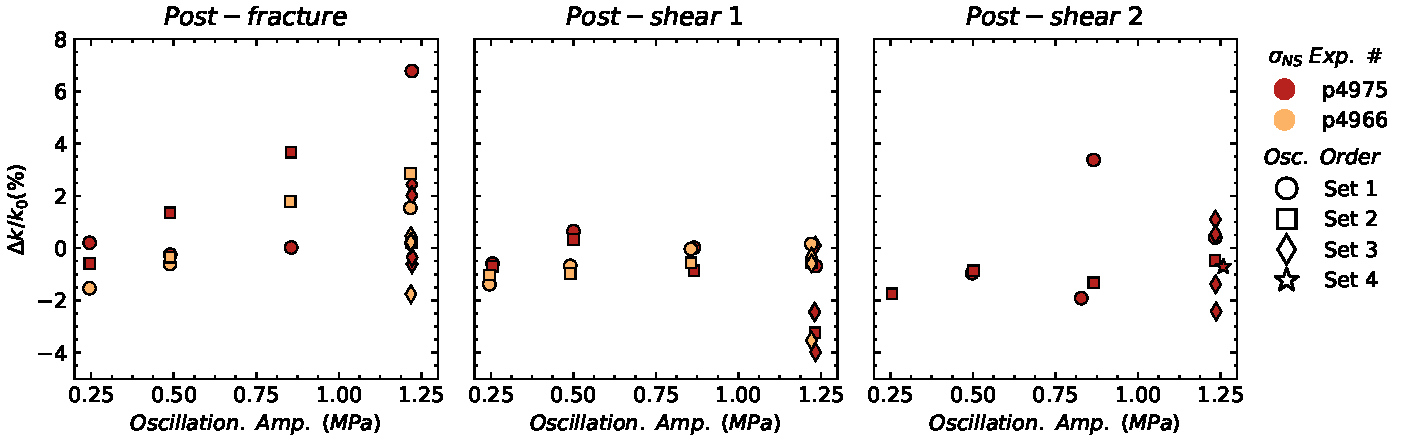
\includegraphics[width=1\columnwidth]{delk_amp_NS}
	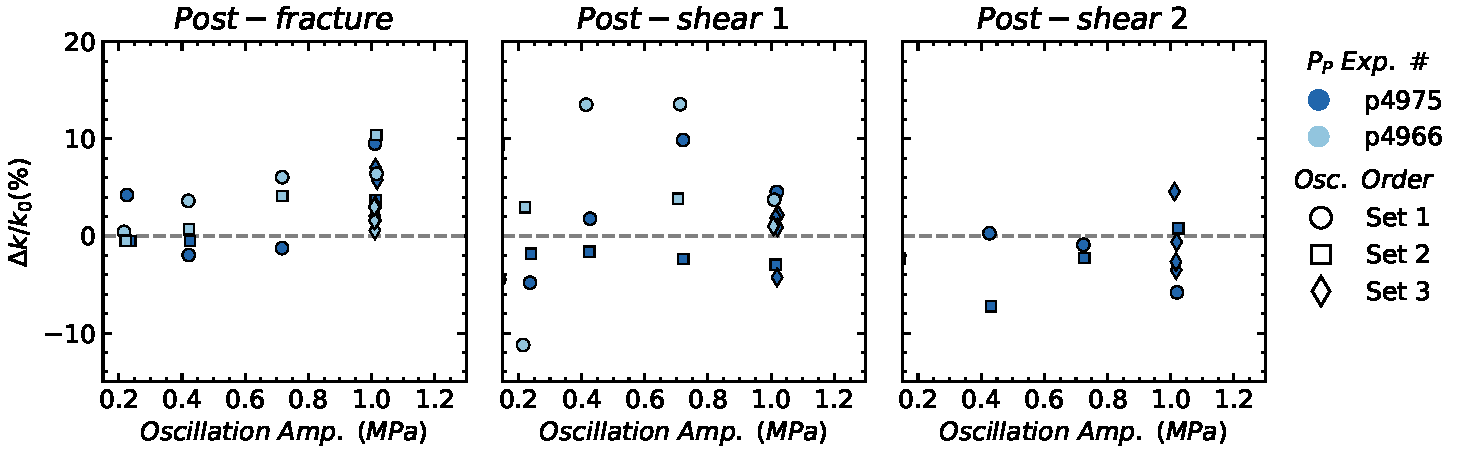
\includegraphics[width=1\columnwidth]{delk_amp_PP}
	%\enspace
	%\includegraphics[width=6cm]{post-frac_amp_array}
	\caption{Change in permeability as a function of $ \sigma_{NS} $ oscillation amplitude. Transitioning from post-fracture results to post-shear results, we observe decreased nonlinearity and permeability enhancement. This is probably related to clogging mechanisms.}%
	\label{fig:perm_ns_amp}
\end{figure}

\newpage

\begin{figure}[ht]
	\centering
	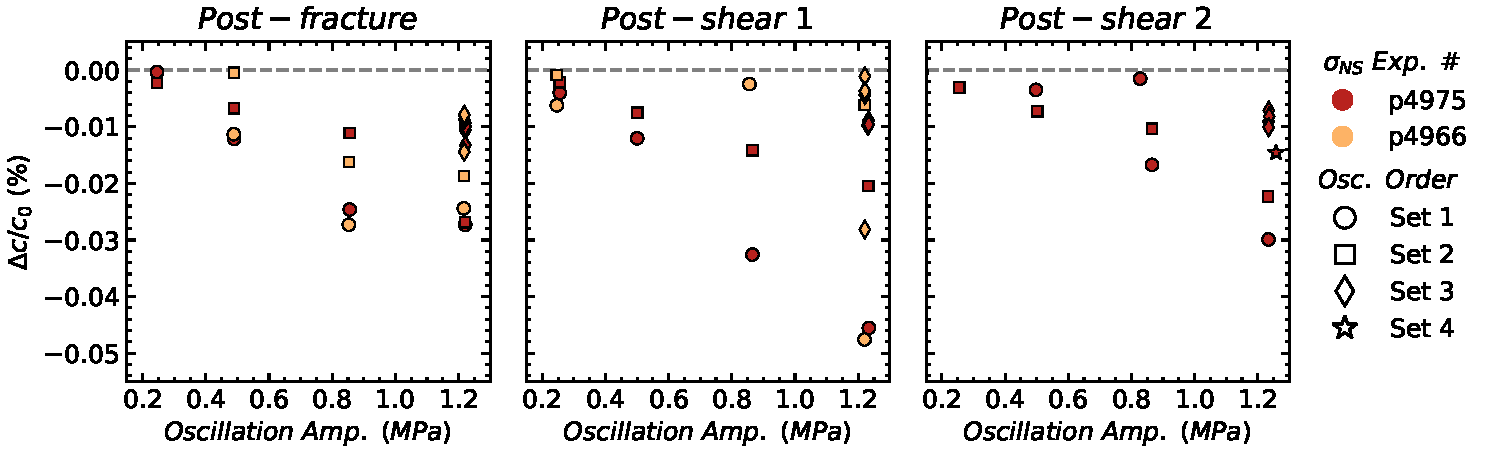
\includegraphics[width=1\columnwidth]{delc_amp_NS}
	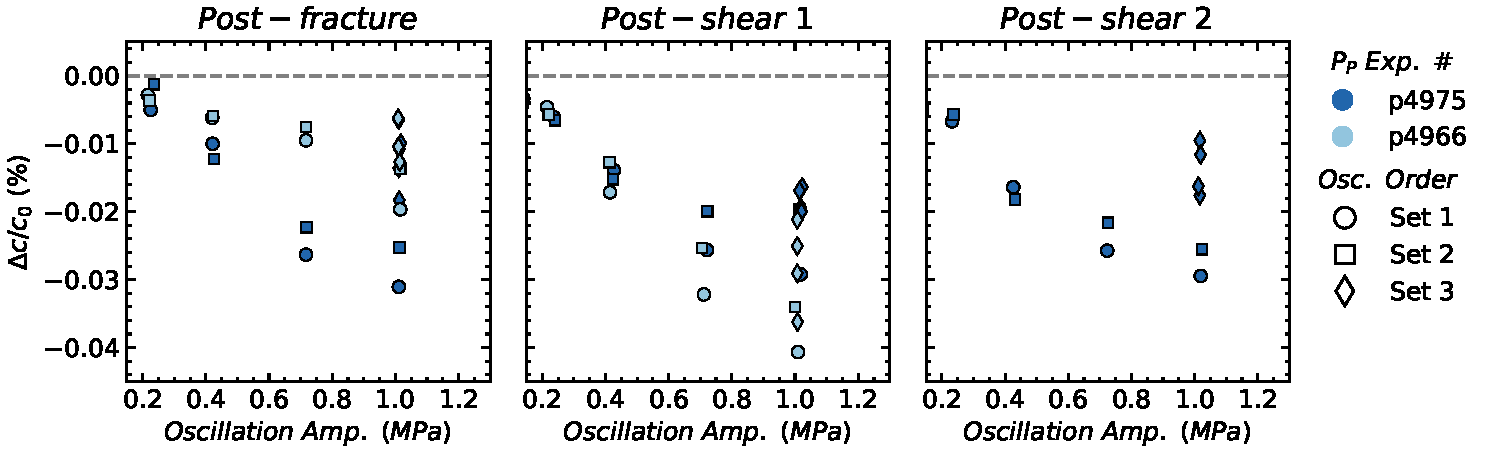
\includegraphics[width=1\columnwidth]{delc_amp_PP}
	%\enspace
	%\includegraphics[width=6cm]{post-frac_amp_array}
	\caption{Nonlinearity as a function of $ \sigma_{NS} $ oscillation amplitude. Transitioning from post-fracture results to post-shear results, we observe decreased nonlinearity and permeability enhancement. This is probably related to clogging mechanisms.}%
	\label{fig:delc_ns_amp}
\end{figure}

\newpage

%\subsection{Relative Change in Velocity and Permeability: Ray Paths}

\begin{figure}[ht]
	\centering
	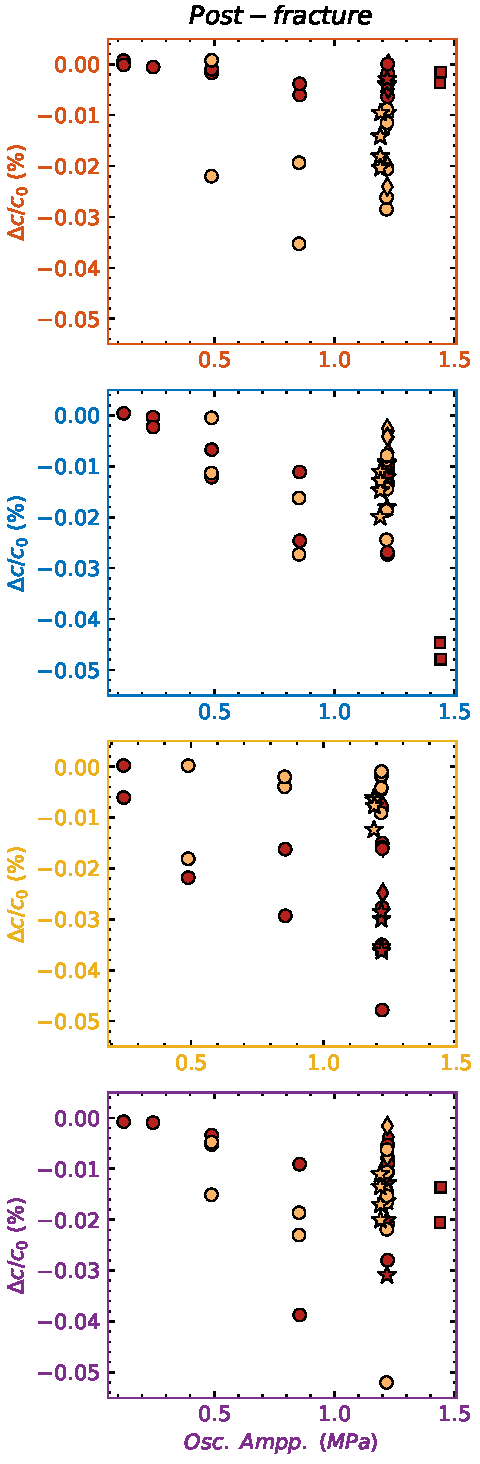
\includegraphics[width=0.31\columnwidth]{Delc_bypair_f_NS}
	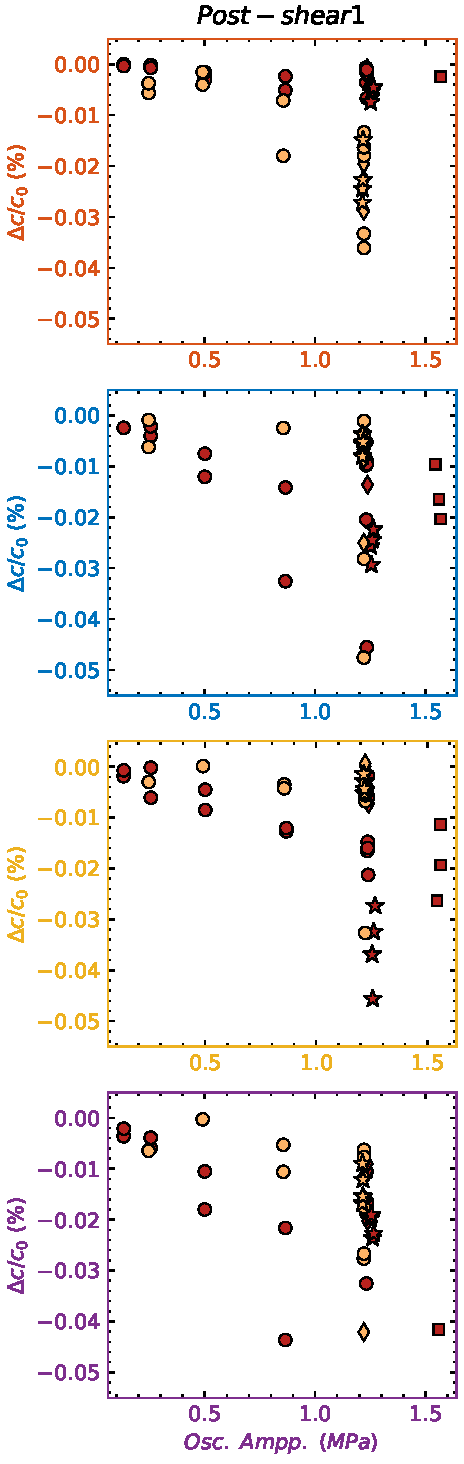
\includegraphics[width=0.3\columnwidth]{Delc_bypair_s1_NS}
	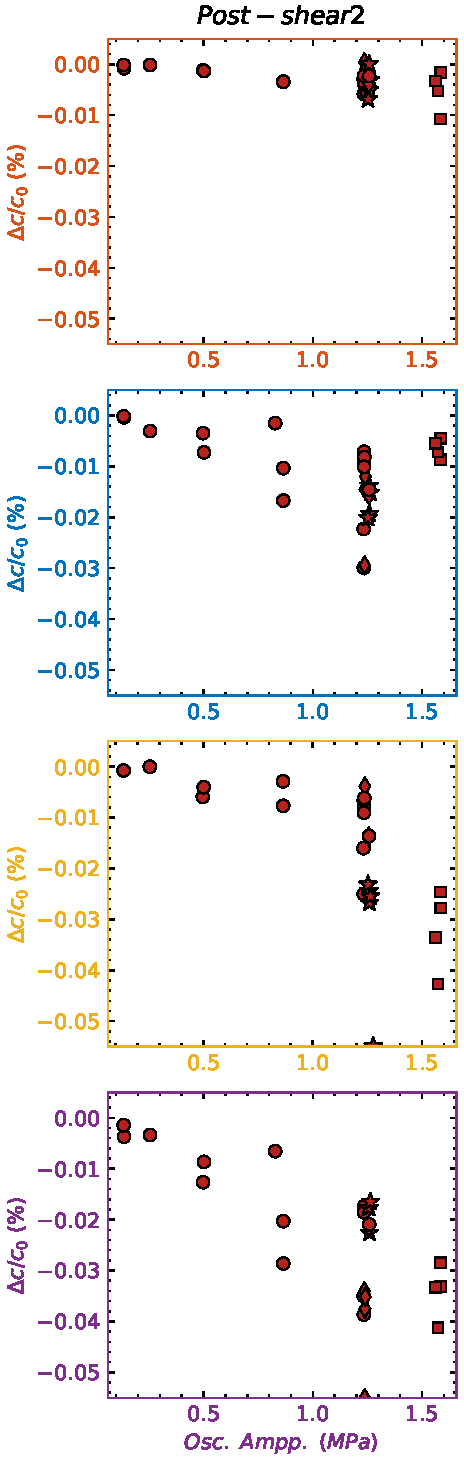
\includegraphics[width=0.3\columnwidth]{Delc_bypair_s2_NS}
	%\enspace
	%\includegraphics[width=6cm]{post-frac_amp_array}
	\caption{Nonlinearity as a function of permeability change for $ \sigma_{NS} $ oscillations for each receiver. Transitioning from post-fracture results to post-shear results, we observe decreased nonlinearity and permeability enhancement. \textbf{\textit{Must insert ray path diagram!!}}}%
	%	\label{fig:delc_plots_ns}
\end{figure}

\newpage


\begin{figure}[ht]
	\centering
	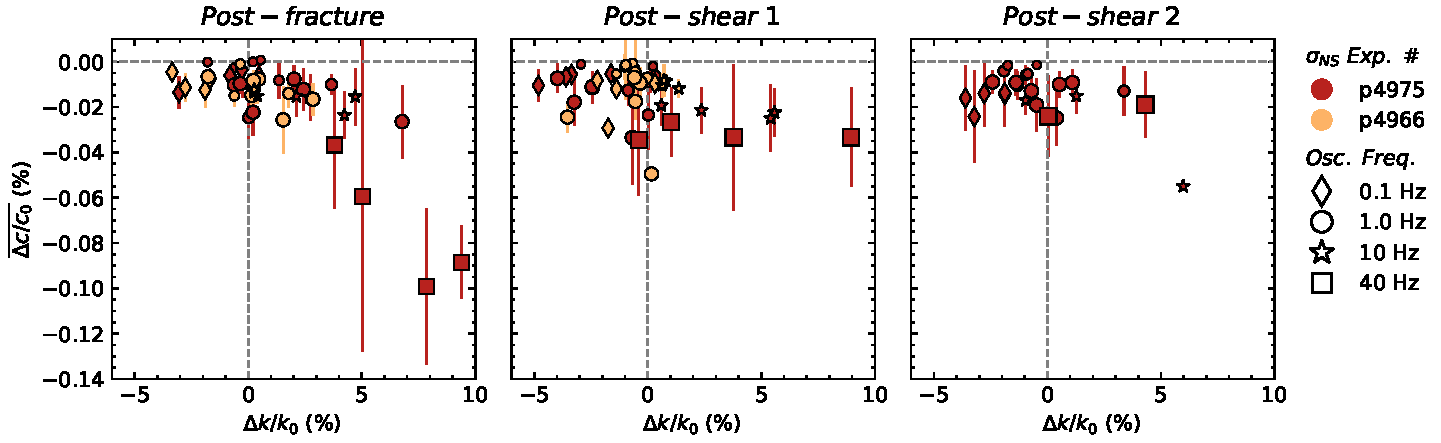
\includegraphics[width=1\columnwidth]{avgDelc_All_ampsNS}
	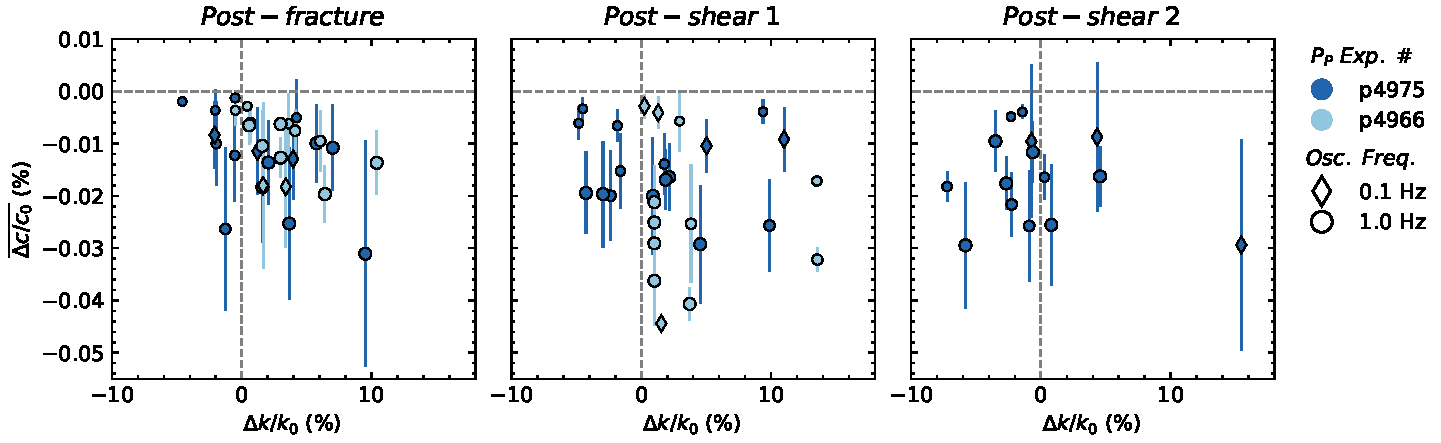
\includegraphics[width=1\columnwidth]{avgDelc_All_ampsPP}
	%\enspace
	%\includegraphics[width=6cm]{post-frac_amp_array}
	\caption{Nonlinearity as a function of permeability change for $ \sigma_{NS} $ and $ P_P $ oscillations averaged over all receivers. Permeability is an averaged measurement across the fracture, so these parameters should exhibit some relationship. I don’t know what this says about the mechanisms at play. Maybe the contact area has been reduced (lower nonlin) and also maybe wear material was mobilized during Pp oscillation sand temporarily increased contact area (higher nonlin). Does this match with reality -- does shearing the fracture increase the contact area? My intuition agrees with this, but it is conceivable that with a complex geometry, this could be more complex.}
	\label{fig:delc_plots2}
\end{figure}

\newpage


\subsection{Nonlinear Elastodynamic Response: Relative Change in RMS Amplitude}

\begin{figure}[ht]
	\centering
	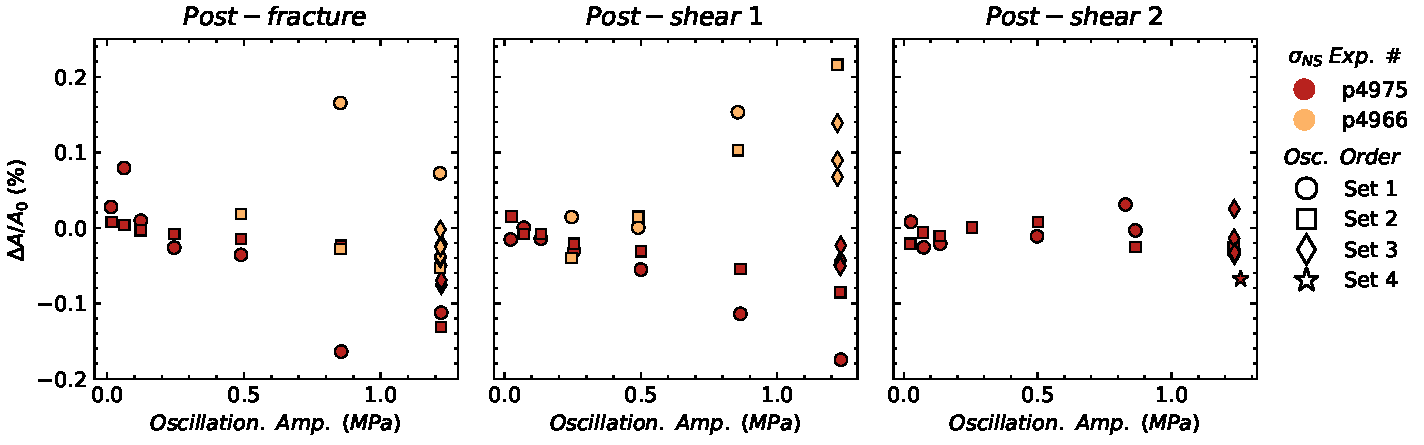
\includegraphics[width=1\columnwidth]{delA_amp_NS}
	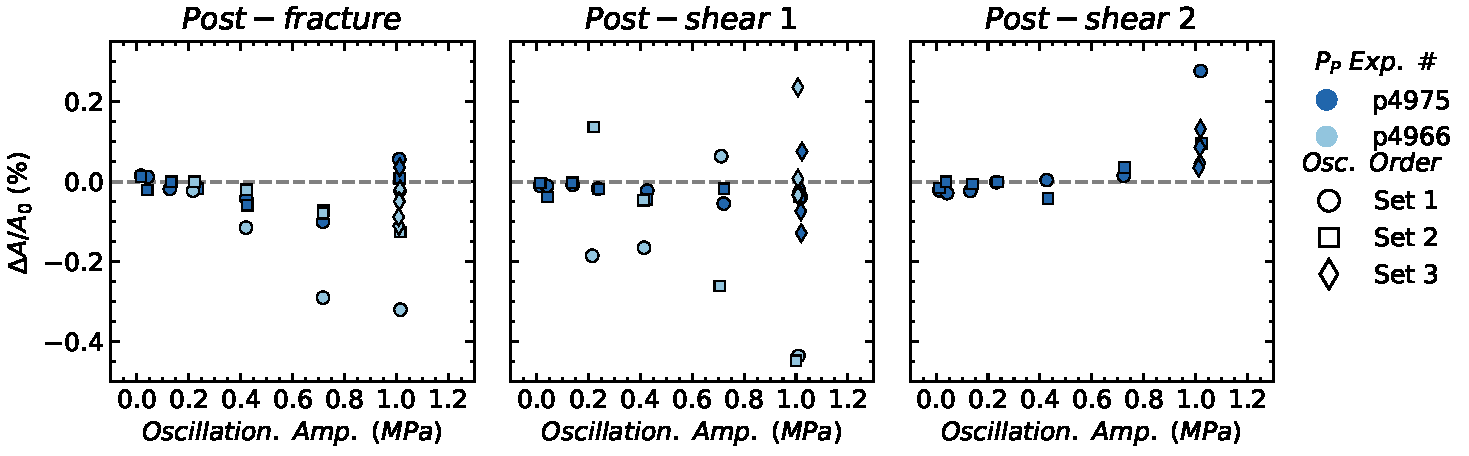
\includegraphics[width=1\columnwidth]{delA_amp_PP}
	%\enspace
	%\includegraphics[width=6cm]{post-frac_amp_array}
	\caption{Nonlinearity as a function of $ \sigma_{NS} $ oscillation amplitude. Transitioning from post-fracture results to post-shear results, we observe decreased nonlinearity and permeability enhancement. This is probably related to clogging mechanisms.}%
	\label{fig:delA_ns_amp}
\end{figure}

\newpage


\begin{figure}[ht]
	\centering
	\includegraphics[width=1\columnwidth]{avg_DelA_perm_NS}
	\includegraphics[width=1\columnwidth]{avg_DelA_perm_PP}
	%\enspace
	%\includegraphics[width=6cm]{post-frac_amp_array}
	\caption{Nonlinearity as a function of permeability change for $ \sigma_{NS} $ and $ P_P $ oscillations averaged over all receivers. Permeability is an averaged measurement across the fracture, so these parameters should exhibit some relationship. I don’t know what this says about the mechanisms at play. Maybe the contact area has been reduced (lower nonlin) and also maybe wear material was mobilized during Pp oscillation sand temporarily increased contact area (higher nonlin). Does this match with reality -- does shearing the fracture increase the contact area? My intuition agrees with this, but it is conceivable that with a complex geometry, this could be more complex.}
	\label{fig:dela_plots2}
\end{figure}

\newpage

\subsection{Velocity Amplitude Modulation during Oscillations}




\begin{itemize}
	\item Although the origins of $dc/c_0 $ and $ dc/c $ remain unclear, consider empirical evidence from [Rivière et al., 2015, 2016] that they originate from different micro-scale mechanisms 
\end{itemize}


\begin{figure}[ht]
	\centering
	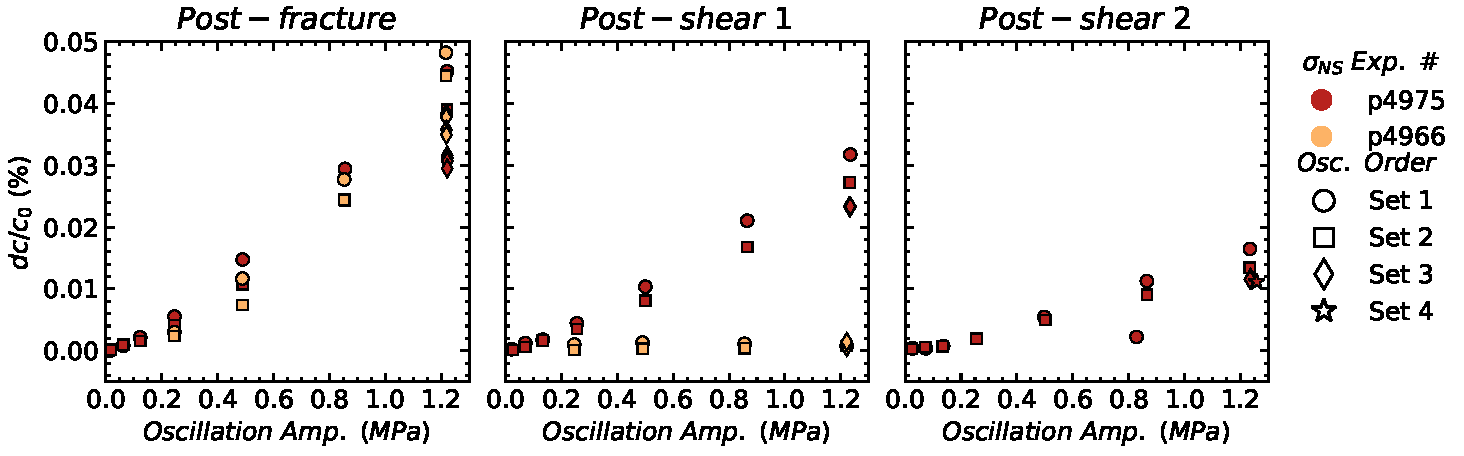
\includegraphics[width=1\columnwidth]{dc_amp_NS}
	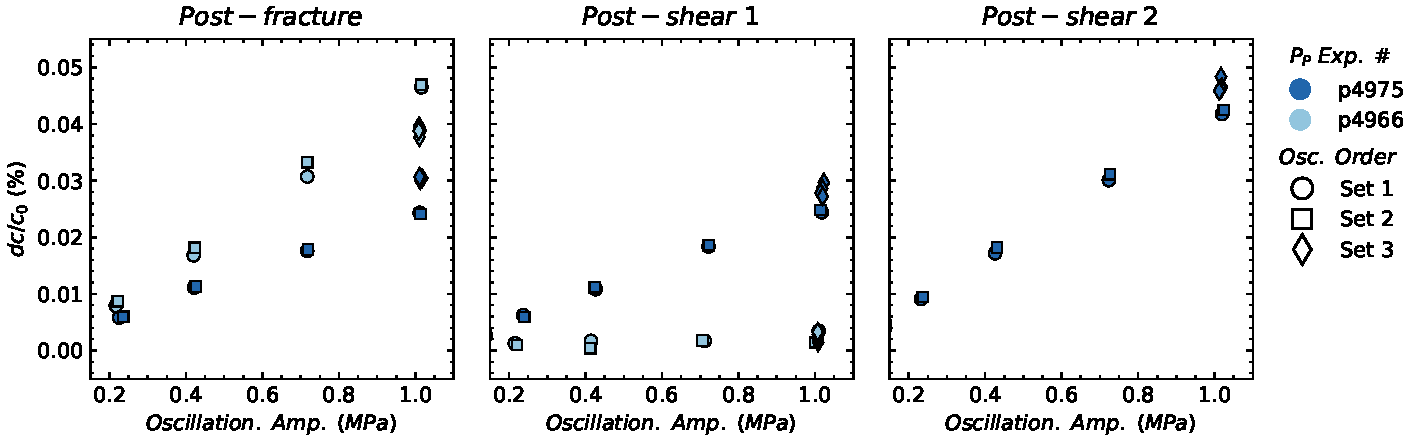
\includegraphics[width=1\columnwidth]{dc_amp_PP}
	%\enspace
	%\includegraphics[width=6cm]{post-frac_amp_array}
	\caption{Velocity amplitude modulation averaged over all receivers ($ dc/c_0 $) as a function of permeability recovery ($ \dot k $) for NS and PP oscillations. 
		I suspect that the we are not waiting long enough to see a trend like J. Elkhoury and others. His recovery values were ~0.5, which he says is related to the dimensionality of the fracture. Shearing the fracture increases the complexity and maybe changes the slope -- dominated by clogging/moving wear material rather than mated aperture.}
	\label{fig:dc_plots2}
\end{figure}

\newpage

%\subsection{Recovery of Velocity and Permeability}
%\begin{itemize}
%	\item Although the origins of $ \Delta c/c_0 $ and $ dc/c $ remain unclear, consider empirical evidence from [Rivière et al., 2015, 2016] that they originate from different micro-scale mechanisms 
%\end{itemize}
%
%
%\begin{figure}[ht]
%	\centering
%%	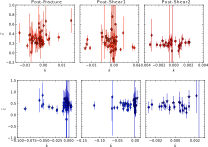
\includegraphics[width=1\columnwidth]{avgRecovBoth_NSPP}
%	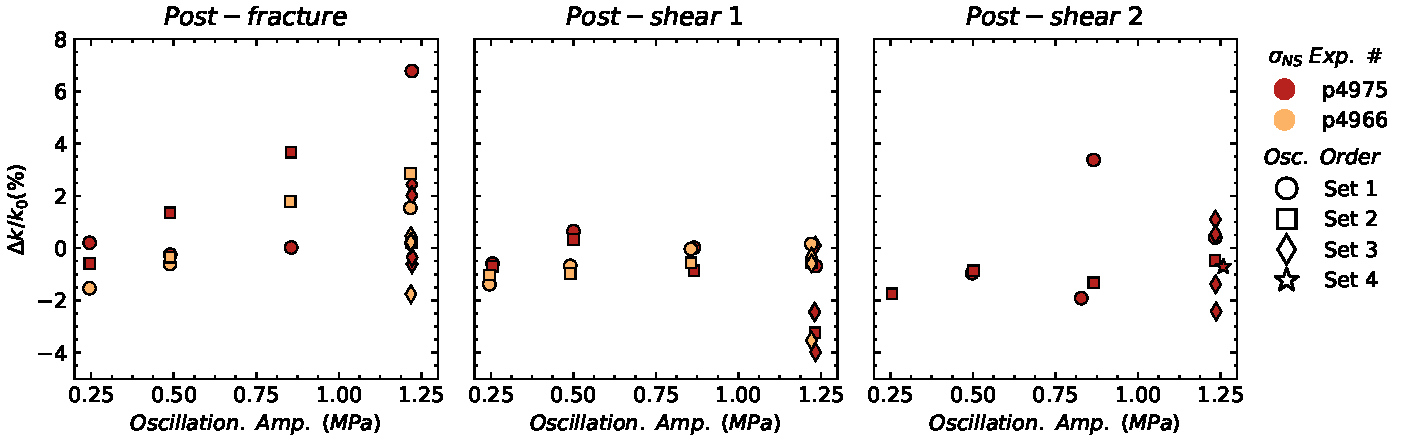
\includegraphics[width=1\columnwidth]{delk_amp_NS}
%	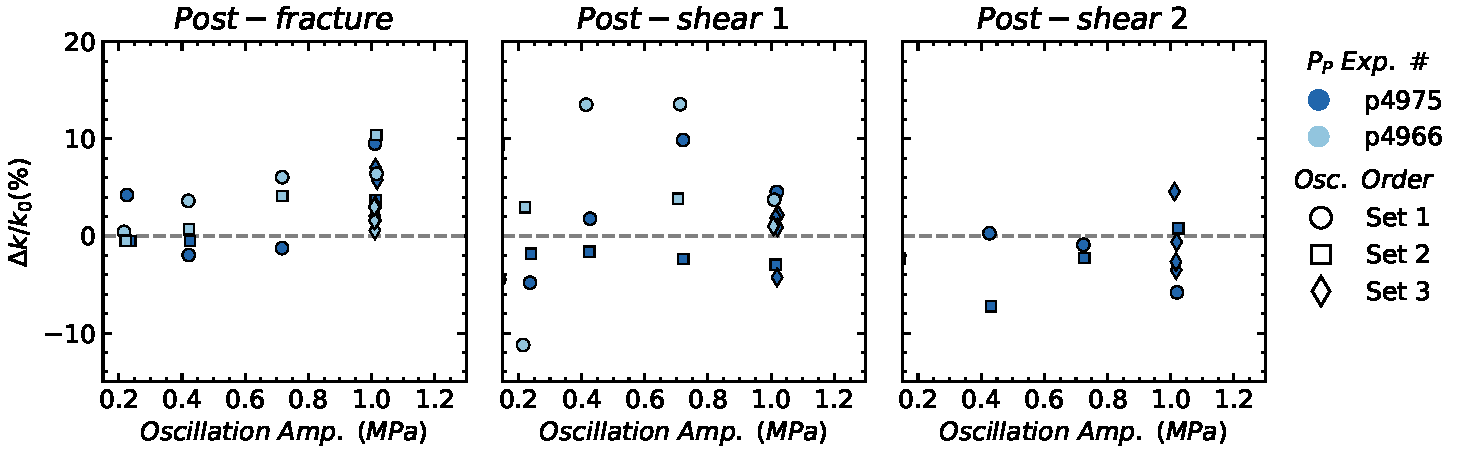
\includegraphics[width=1\columnwidth]{delk_amp_PP}
%	%\enspace
%	%\includegraphics[width=6cm]{post-frac_amp_array}
%	\caption{Velocity recovery averaged over all receivers ($ \overline {\dot c} $) as a function of oscillation amplitude for NS and PP oscillations. 
%	I suspect that the we are not waiting long enough to see a trend like J. Elkhoury and others. His recovery values were ~0.5, which he says is related to the dimensionality of the fracture. Shearing the fracture increases the complexity and maybe changes the slope -- dominated by clogging/moving wear material rather than mated aperture.}
%	\label{fig:cdot_amp}
%\end{figure}
%
%\newpage


%\begin{figure}[ht]
%	\centering
%	%	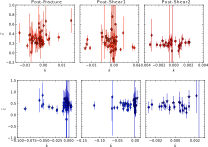
\includegraphics[width=1\columnwidth]{avgRecovBoth_NSPP}
%	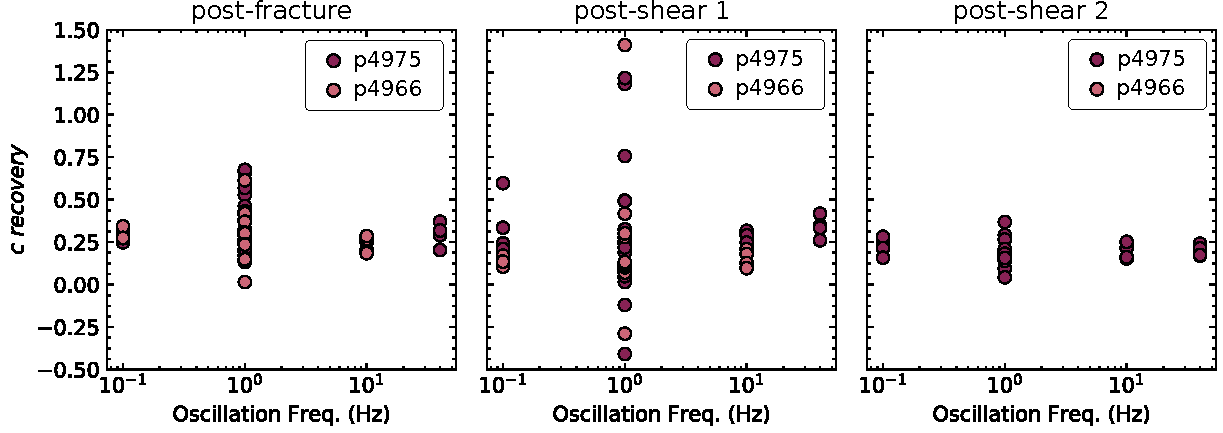
\includegraphics[width=1\columnwidth]{Cdot_NS_freq}
%	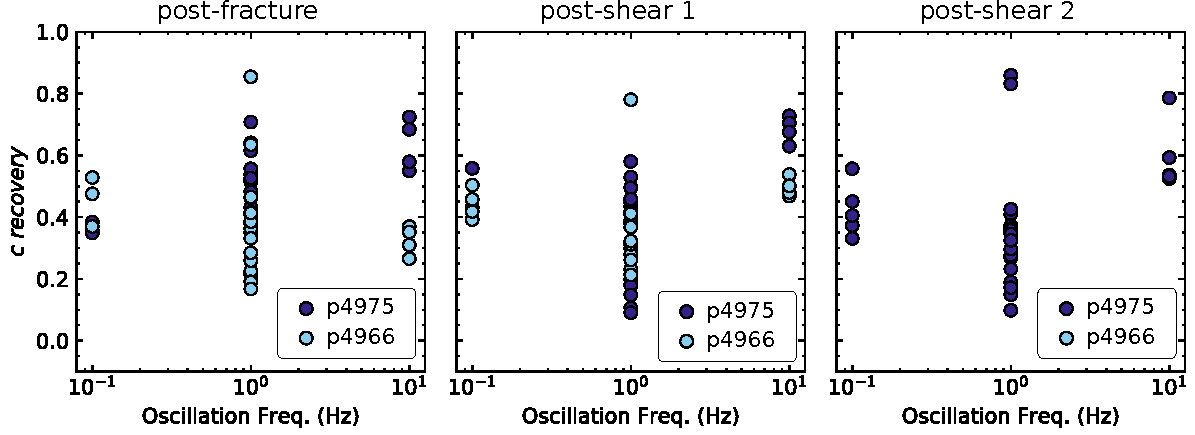
\includegraphics[width=1\columnwidth]{Cdot_PP_freq}
%	%\enspace
%	%\includegraphics[width=6cm]{post-frac_amp_array}
%	\caption{Velocity recovery averaged over all receivers ($ \overline {\dot c} $) as a function of oscillation frequency for NS and PP oscillations. 
%		I suspect that the we are not waiting long enough to see a trend like J. Elkhoury and others. His recovery values were ~0.5, which he says is related to the dimensionality of the fracture. Shearing the fracture increases the complexity and maybe changes the slope -- dominated by clogging/moving wear material rather than mated aperture.}
%	\label{fig:cdot_amp}
%\end{figure}

\newpage

%\subsection{Effect of Fracture Aperture}
%\begin{itemize}
%	\item effect of fracture aperture modulated by shearing the fractured samples in two 5mm increments, repeating the dynamic stressing protocols. Elucidates how changes in the aperture size distribution due to shearing and wear–alter the fracture stiffness and the stress-dependency.
%	\item shearing of the fracture reduces the nonlinearity measured during normal stress oscillations
%	\item oscillations become generally less effective in enhancing the fracture permeability.
%	\item the correlation between the nonlinearity and permeability change and sample thickness change is stronger for NS oscillations than Pp. 
%	\item There is no clear correlation between perm change and flow rate during oscillations, suggesting “unclogging” may not be the sole mechanism responsible for perm change due to Pp oscillations. 
%	\item However, we report nonlinearity after the second shear history: indicative of possible differences in mechanisms activated during the two modes of stressing.
%\end{itemize}
%
%\newpage